\documentclass[a4paper]{book}
\usepackage{a4wide}
\usepackage{makeidx}
\usepackage{graphicx}
\usepackage{multicol}
\usepackage{float}
\usepackage{listings}
\usepackage{color}
\usepackage{textcomp}
\usepackage{alltt}
\usepackage{times}
\usepackage{ifpdf}
\ifpdf
\usepackage[pdftex,
            pagebackref=true,
            colorlinks=true,
            linkcolor=blue,
            unicode
           ]{hyperref}
\else
\usepackage[ps2pdf,
            pagebackref=true,
            colorlinks=true,
            linkcolor=blue,
            unicode
           ]{hyperref}
\usepackage{pspicture}
\fi
\usepackage[utf8]{inputenc}
\usepackage{doxygen}
\lstset{language=C++,inputencoding=utf8,basicstyle=\footnotesize,breaklines=true,breakatwhitespace=true,tabsize=8,numbers=left }
\makeindex
\setcounter{tocdepth}{3}
\renewcommand{\footrulewidth}{0.4pt}
\begin{document}
\hypersetup{pageanchor=false}
\begin{titlepage}
\vspace*{7cm}
\begin{center}
{\Large ReuseDistance \\[1ex]\large 0.01 }\\
\vspace*{1cm}
{\large Generated by Doxygen 1.6.3}\\
\vspace*{0.5cm}
{\small Sun Oct 21 14:56:27 2012}\\
\end{center}
\end{titlepage}
\clearemptydoublepage
\pagenumbering{roman}
\tableofcontents
\clearemptydoublepage
\pagenumbering{arabic}
\hypersetup{pageanchor=true}
\chapter{Class Index}
\section{Class Hierarchy}
This inheritance list is sorted roughly, but not completely, alphabetically:\begin{DoxyCompactList}
\item \contentsline{section}{node234\_\-Tag}{\pageref{structnode234___tag}}{}
\item \contentsline{section}{ReuseDistance}{\pageref{class_reuse_distance}}{}
\begin{DoxyCompactList}
\item \contentsline{section}{SpatialLocality}{\pageref{class_spatial_locality}}{}
\end{DoxyCompactList}
\item \contentsline{section}{ReuseEntry}{\pageref{struct_reuse_entry}}{}
\item \contentsline{section}{ReuseStats}{\pageref{class_reuse_stats}}{}
\item \contentsline{section}{tree234\_\-Tag}{\pageref{structtree234___tag}}{}
\end{DoxyCompactList}

\chapter{Class Index}
\section{Class List}
Here are the classes, structs, unions and interfaces with brief descriptions:\begin{DoxyCompactList}
\item\contentsline{section}{\hyperlink{structnode234___tag}{node234\_\-Tag} }{\pageref{structnode234___tag}}{}
\item\contentsline{section}{\hyperlink{class_reuse_distance}{ReuseDistance} }{\pageref{class_reuse_distance}}{}
\item\contentsline{section}{\hyperlink{struct_reuse_entry}{ReuseEntry} }{\pageref{struct_reuse_entry}}{}
\item\contentsline{section}{\hyperlink{class_reuse_stats}{ReuseStats} }{\pageref{class_reuse_stats}}{}
\item\contentsline{section}{\hyperlink{class_spatial_locality}{SpatialLocality} }{\pageref{class_spatial_locality}}{}
\item\contentsline{section}{\hyperlink{structtree234___tag}{tree234\_\-Tag} }{\pageref{structtree234___tag}}{}
\end{DoxyCompactList}

\chapter{File Index}
\section{File List}
Here is a list of all files with brief descriptions:\begin{DoxyCompactList}
\item\contentsline{section}{/home/michaell/software/ReuseDistance/\hyperlink{foo_8cpp}{foo.cpp} }{\pageref{foo_8cpp}}{}
\item\contentsline{section}{/home/michaell/software/ReuseDistance/\hyperlink{_reuse_distance_8cpp}{ReuseDistance.cpp} }{\pageref{_reuse_distance_8cpp}}{}
\item\contentsline{section}{/home/michaell/software/ReuseDistance/\hyperlink{_reuse_distance_8hpp}{ReuseDistance.hpp} }{\pageref{_reuse_distance_8hpp}}{}
\item\contentsline{section}{/home/michaell/software/ReuseDistance/\hyperlink{tree234_8c}{tree234.c} }{\pageref{tree234_8c}}{}
\item\contentsline{section}{/home/michaell/software/ReuseDistance/\hyperlink{tree234_8h}{tree234.h} }{\pageref{tree234_8h}}{}
\end{DoxyCompactList}

\chapter{Class Documentation}
\hypertarget{structnode234___tag}{
\section{node234\_\-Tag Struct Reference}
\label{structnode234___tag}\index{node234\_\-Tag@{node234\_\-Tag}}
}
\subsection*{Public Attributes}
\begin{DoxyCompactItemize}
\item 
\hyperlink{structnode234___tag}{node234} $\ast$ \hyperlink{structnode234___tag_a3c3bdead5844de4df21b2980e7409157}{parent}
\item 
\hyperlink{structnode234___tag}{node234} $\ast$ \hyperlink{structnode234___tag_a0f783514c021d86027beb3211b43f3b7}{kids} \mbox{[}4\mbox{]}
\item 
int \hyperlink{structnode234___tag_a06142da7798558b8c6d59d1cb6471a10}{counts} \mbox{[}4\mbox{]}
\item 
\hyperlink{struct_reuse_entry}{ReuseEntry} $\ast$ \hyperlink{structnode234___tag_a55c085a9b0e3812d029a17f366e274f7}{elems} \mbox{[}3\mbox{]}
\end{DoxyCompactItemize}


\subsection{Detailed Description}


Definition at line 58 of file tree234.c.



\subsection{Member Data Documentation}
\hypertarget{structnode234___tag_a06142da7798558b8c6d59d1cb6471a10}{
\index{node234\_\-Tag@{node234\_\-Tag}!counts@{counts}}
\index{counts@{counts}!node234_Tag@{node234\_\-Tag}}
\subsubsection[{counts}]{\setlength{\rightskip}{0pt plus 5cm}int {\bf node234\_\-Tag::counts}\mbox{[}4\mbox{]}}}
\label{structnode234___tag_a06142da7798558b8c6d59d1cb6471a10}


Definition at line 61 of file tree234.c.

\hypertarget{structnode234___tag_a55c085a9b0e3812d029a17f366e274f7}{
\index{node234\_\-Tag@{node234\_\-Tag}!elems@{elems}}
\index{elems@{elems}!node234_Tag@{node234\_\-Tag}}
\subsubsection[{elems}]{\setlength{\rightskip}{0pt plus 5cm}{\bf ReuseEntry}$\ast$ {\bf node234\_\-Tag::elems}\mbox{[}3\mbox{]}}}
\label{structnode234___tag_a55c085a9b0e3812d029a17f366e274f7}


Definition at line 62 of file tree234.c.

\hypertarget{structnode234___tag_a0f783514c021d86027beb3211b43f3b7}{
\index{node234\_\-Tag@{node234\_\-Tag}!kids@{kids}}
\index{kids@{kids}!node234_Tag@{node234\_\-Tag}}
\subsubsection[{kids}]{\setlength{\rightskip}{0pt plus 5cm}{\bf node234}$\ast$ {\bf node234\_\-Tag::kids}\mbox{[}4\mbox{]}}}
\label{structnode234___tag_a0f783514c021d86027beb3211b43f3b7}


Definition at line 60 of file tree234.c.

\hypertarget{structnode234___tag_a3c3bdead5844de4df21b2980e7409157}{
\index{node234\_\-Tag@{node234\_\-Tag}!parent@{parent}}
\index{parent@{parent}!node234_Tag@{node234\_\-Tag}}
\subsubsection[{parent}]{\setlength{\rightskip}{0pt plus 5cm}{\bf node234}$\ast$ {\bf node234\_\-Tag::parent}}}
\label{structnode234___tag_a3c3bdead5844de4df21b2980e7409157}


Definition at line 59 of file tree234.c.



The documentation for this struct was generated from the following file:\begin{DoxyCompactItemize}
\item 
/home/michaell/software/ReuseDistance/\hyperlink{tree234_8c}{tree234.c}\end{DoxyCompactItemize}

\hypertarget{class_reuse_distance}{
\section{ReuseDistance Class Reference}
\label{class_reuse_distance}\index{ReuseDistance@{ReuseDistance}}
}


{\ttfamily \#include $<$ReuseDistance.hpp$>$}

Inheritance diagram for ReuseDistance:\begin{figure}[H]
\begin{center}
\leavevmode
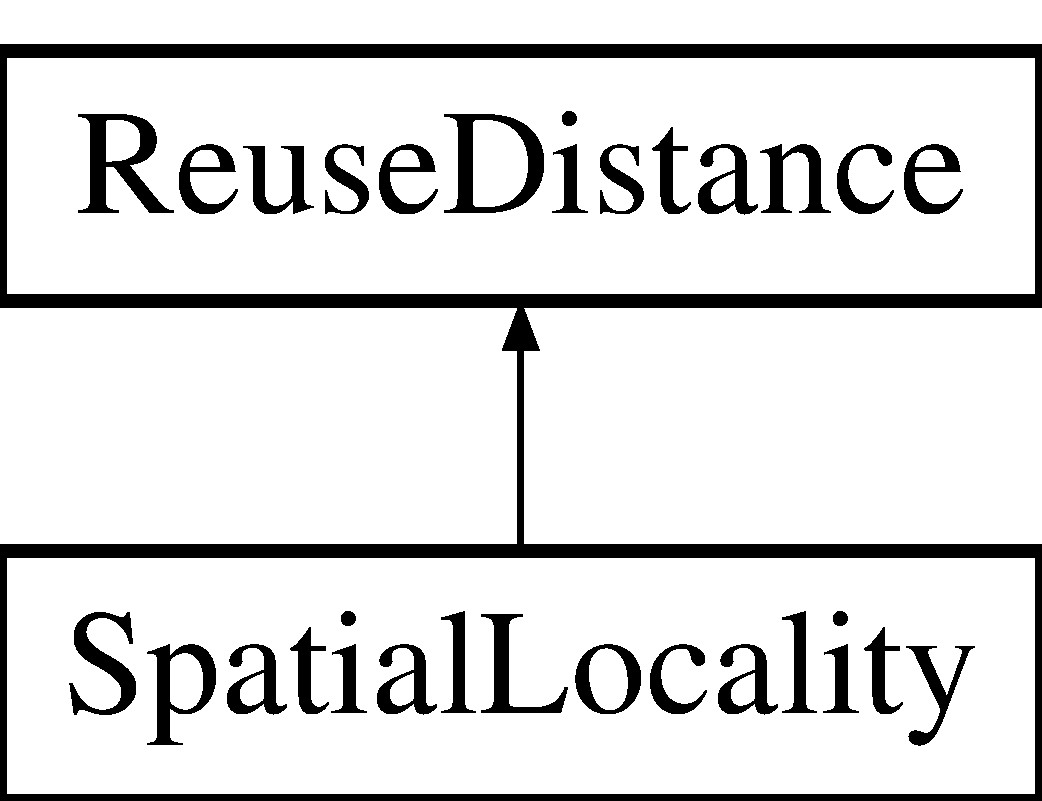
\includegraphics[height=2cm]{class_reuse_distance}
\end{center}
\end{figure}
\subsection*{Public Member Functions}
\begin{DoxyCompactItemize}
\item 
\hyperlink{class_reuse_distance_a0248afa697da0f6c87c6fd30c289ecc6}{ReuseDistance} (uint64\_\-t w, uint64\_\-t b)
\item 
\hyperlink{class_reuse_distance_ab68a2d9df5c28571c3f8820c5344b2c1}{ReuseDistance} (uint64\_\-t w)
\item 
virtual \hyperlink{class_reuse_distance_a2846a6f2c045759657b754838045900d}{$\sim$ReuseDistance} ()
\item 
virtual void \hyperlink{class_reuse_distance_ae693ec30500fcdd2222f0f07d207c0ce}{Print} (std::ostream \&f, bool annotate=false)
\item 
virtual void \hyperlink{class_reuse_distance_a2ce354238975243f602201787c9282ba}{Print} (bool annotate=false)
\item 
void \hyperlink{class_reuse_distance_a027a92a58a6639e8ed13a7490d11dcf5}{PrintFormat} (std::ostream \&f)
\item 
virtual void \hyperlink{class_reuse_distance_a4ff6b77022ce62e0fdefa5cc297b932a}{Process} (\hyperlink{struct_reuse_entry}{ReuseEntry} \&addr)
\item 
void \hyperlink{class_reuse_distance_aed9cbdd99de67972a37de4624614de9d}{Process} (\hyperlink{struct_reuse_entry}{ReuseEntry} $\ast$addrs, uint64\_\-t count)
\item 
void \hyperlink{class_reuse_distance_a372960c10d5fb6552c8dfcfd77da38ba}{Process} (std::vector$<$ \hyperlink{struct_reuse_entry}{ReuseEntry} $>$ rs)
\item 
void \hyperlink{class_reuse_distance_a88052f5ae1e69bab8fe1f9b7b87c1037}{Process} (std::vector$<$ \hyperlink{struct_reuse_entry}{ReuseEntry} $\ast$ $>$ addrs)
\item 
\hyperlink{class_reuse_stats}{ReuseStats} $\ast$ \hyperlink{class_reuse_distance_a771580c25dc5140969919e959e2ebdd1}{GetStats} (uint64\_\-t id)
\item 
void \hyperlink{class_reuse_distance_a99fb4b3aae663676515ad354691b7cc6}{GetIndices} (std::vector$<$ uint64\_\-t $>$ \&ids)
\item 
virtual void \hyperlink{class_reuse_distance_acc4885040a8a518fc10b5aa4da7d777a}{GetActiveAddresses} (std::vector$<$ uint64\_\-t $>$ \&addrs)
\item 
virtual void \hyperlink{class_reuse_distance_a0763528236db14a9e0234465e72da3b6}{SkipAddresses} (uint64\_\-t amount)
\end{DoxyCompactItemize}
\subsection*{Static Public Attributes}
\begin{DoxyCompactItemize}
\item 
static const uint64\_\-t \hyperlink{class_reuse_distance_af0d9cba7105109e89ae6b7177f54c976}{DefaultBinIndividual} = 32
\item 
static const uint64\_\-t \hyperlink{class_reuse_distance_a59f7f0ac6ad014472537619394ac7375}{Infinity} = INFINITY\_\-REUSE
\end{DoxyCompactItemize}
\subsection*{Protected Member Functions}
\begin{DoxyCompactItemize}
\item 
void \hyperlink{class_reuse_distance_a265c98b7a9460b3312ea5c78dae968cc}{Init} (uint64\_\-t w, uint64\_\-t b)
\item 
virtual \hyperlink{class_reuse_stats}{ReuseStats} $\ast$ \hyperlink{class_reuse_distance_adb13097f908e002f1da8e188d7dc3210}{GetStats} (uint64\_\-t id, bool gen)
\item 
virtual const std::string \hyperlink{class_reuse_distance_a6ef63a5e5b15c5dce387e026d40d6ef2}{Describe} ()
\end{DoxyCompactItemize}
\subsection*{Protected Attributes}
\begin{DoxyCompactItemize}
\item 
reuse\_\-map\_\-type$<$ uint64\_\-t, \hyperlink{class_reuse_stats}{ReuseStats} $\ast$ $>$ \hyperlink{class_reuse_distance_a37e4f6796798fe8839e94c956b4354ee}{stats}
\item 
uint64\_\-t \hyperlink{class_reuse_distance_a8e3536264e92460f10455af7f1e161fd}{capacity}
\item 
uint64\_\-t \hyperlink{class_reuse_distance_a5d38c22d7841765630b828eed50ac345}{sequence}
\item 
uint64\_\-t \hyperlink{class_reuse_distance_a62dae87cc1183b8bcbfa2220ddd9a3e2}{binindividual}
\item 
uint64\_\-t \hyperlink{class_reuse_distance_ac3e8daa6fa8c16cdf955fd6cf99ba932}{maxtracking}
\end{DoxyCompactItemize}


\subsection{Detailed Description}
Tracks reuse distances for a memory address stream. Keep track of the addresses within a specific window of history, whose size can be finite or infinite. For basic usage, see the documentation at \href{http://bit.ly/ScqZVj}{\tt http://bit.ly/ScqZVj} for the constructors, the Process methods and the Print methods. Also see the simple test file test/test.cpp included in this source package. 

Definition at line 86 of file ReuseDistance.hpp.



\subsection{Constructor \& Destructor Documentation}
\hypertarget{class_reuse_distance_a0248afa697da0f6c87c6fd30c289ecc6}{
\index{ReuseDistance@{ReuseDistance}!ReuseDistance@{ReuseDistance}}
\index{ReuseDistance@{ReuseDistance}!ReuseDistance@{ReuseDistance}}
\subsubsection[{ReuseDistance}]{\setlength{\rightskip}{0pt plus 5cm}ReuseDistance::ReuseDistance (uint64\_\-t {\em w}, \/  uint64\_\-t {\em b})}}
\label{class_reuse_distance_a0248afa697da0f6c87c6fd30c289ecc6}
Contructs a \hyperlink{class_reuse_distance}{ReuseDistance} object.


\begin{DoxyParams}{Parameters}
\item[{\em w}]The maximum window size, or alternatively the maximum possible reuse distance that this tool will find. No window/distance limit is imposed if \hyperlink{class_reuse_distance_a59f7f0ac6ad014472537619394ac7375}{ReuseDistance::Infinity} is used, though you could easily run of of memory. \item[{\em b}]All distances not greater than b will be tracked individually. All distances are tracked individually if b == \hyperlink{class_reuse_distance_a59f7f0ac6ad014472537619394ac7375}{ReuseDistance::Infinity}. Beyond individual tracking, distances are tracked in bins whose boundaries are the powers of two greater than b (and not exeeding w, of course). \end{DoxyParams}


Definition at line 56 of file ReuseDistance.cpp.

\hypertarget{class_reuse_distance_ab68a2d9df5c28571c3f8820c5344b2c1}{
\index{ReuseDistance@{ReuseDistance}!ReuseDistance@{ReuseDistance}}
\index{ReuseDistance@{ReuseDistance}!ReuseDistance@{ReuseDistance}}
\subsubsection[{ReuseDistance}]{\setlength{\rightskip}{0pt plus 5cm}ReuseDistance::ReuseDistance (uint64\_\-t {\em w})}}
\label{class_reuse_distance_ab68a2d9df5c28571c3f8820c5344b2c1}
Contructs a \hyperlink{class_reuse_distance}{ReuseDistance} object. Equivalent to calling the other constructor with b == \hyperlink{class_reuse_distance_af0d9cba7105109e89ae6b7177f54c976}{ReuseDistance::DefaultBinIndividual} 

Definition at line 60 of file ReuseDistance.cpp.

\hypertarget{class_reuse_distance_a2846a6f2c045759657b754838045900d}{
\index{ReuseDistance@{ReuseDistance}!$\sim$ReuseDistance@{$\sim$ReuseDistance}}
\index{$\sim$ReuseDistance@{$\sim$ReuseDistance}!ReuseDistance@{ReuseDistance}}
\subsubsection[{$\sim$ReuseDistance}]{\setlength{\rightskip}{0pt plus 5cm}ReuseDistance::$\sim$ReuseDistance ()\hspace{0.3cm}{\ttfamily  \mbox{[}virtual\mbox{]}}}}
\label{class_reuse_distance_a2846a6f2c045759657b754838045900d}
Destroys a \hyperlink{class_reuse_distance}{ReuseDistance} object. 

Definition at line 64 of file ReuseDistance.cpp.



\subsection{Member Function Documentation}
\hypertarget{class_reuse_distance_a6ef63a5e5b15c5dce387e026d40d6ef2}{
\index{ReuseDistance@{ReuseDistance}!Describe@{Describe}}
\index{Describe@{Describe}!ReuseDistance@{ReuseDistance}}
\subsubsection[{Describe}]{\setlength{\rightskip}{0pt plus 5cm}virtual const std::string ReuseDistance::Describe ()\hspace{0.3cm}{\ttfamily  \mbox{[}inline, protected, virtual\mbox{]}}}}
\label{class_reuse_distance_a6ef63a5e5b15c5dce387e026d40d6ef2}


Definition at line 108 of file ReuseDistance.hpp.

\hypertarget{class_reuse_distance_acc4885040a8a518fc10b5aa4da7d777a}{
\index{ReuseDistance@{ReuseDistance}!GetActiveAddresses@{GetActiveAddresses}}
\index{GetActiveAddresses@{GetActiveAddresses}!ReuseDistance@{ReuseDistance}}
\subsubsection[{GetActiveAddresses}]{\setlength{\rightskip}{0pt plus 5cm}void ReuseDistance::GetActiveAddresses (std::vector$<$ uint64\_\-t $>$ \& {\em addrs})\hspace{0.3cm}{\ttfamily  \mbox{[}virtual\mbox{]}}}}
\label{class_reuse_distance_acc4885040a8a518fc10b5aa4da7d777a}
Get a std::vector containing all of the addresses currently in this \hyperlink{class_reuse_distance}{ReuseDistance} object's active window.


\begin{DoxyParams}{Parameters}
\item[{\em addrs}]A std::vector which will contain the addresses. It is an error to pass this vector non-\/empty (that is addrs.size() == 0 is enforced at runtime).\end{DoxyParams}
\begin{DoxyReturn}{Returns}
none 
\end{DoxyReturn}


Reimplemented in \hyperlink{class_spatial_locality_afef7ecfce7f238dbef37499e08edfb98}{SpatialLocality}.



Definition at line 90 of file ReuseDistance.cpp.

\hypertarget{class_reuse_distance_a99fb4b3aae663676515ad354691b7cc6}{
\index{ReuseDistance@{ReuseDistance}!GetIndices@{GetIndices}}
\index{GetIndices@{GetIndices}!ReuseDistance@{ReuseDistance}}
\subsubsection[{GetIndices}]{\setlength{\rightskip}{0pt plus 5cm}void ReuseDistance::GetIndices (std::vector$<$ uint64\_\-t $>$ \& {\em ids})}}
\label{class_reuse_distance_a99fb4b3aae663676515ad354691b7cc6}
Get a std::vector containing all of the unique indices processed by this \hyperlink{class_reuse_distance}{ReuseDistance} object.


\begin{DoxyParams}{Parameters}
\item[{\em ids}]A std::vector which will contain the ids. It is an error to pass this vector non-\/empty (that is addrs.size() == 0 is enforced at runtime).\end{DoxyParams}
\begin{DoxyReturn}{Returns}
none 
\end{DoxyReturn}


Definition at line 82 of file ReuseDistance.cpp.

\hypertarget{class_reuse_distance_a771580c25dc5140969919e959e2ebdd1}{
\index{ReuseDistance@{ReuseDistance}!GetStats@{GetStats}}
\index{GetStats@{GetStats}!ReuseDistance@{ReuseDistance}}
\subsubsection[{GetStats}]{\setlength{\rightskip}{0pt plus 5cm}{\bf ReuseStats} $\ast$ ReuseDistance::GetStats (uint64\_\-t {\em id})}}
\label{class_reuse_distance_a771580c25dc5140969919e959e2ebdd1}
Get the \hyperlink{class_reuse_stats}{ReuseStats} object associated with some unique id.


\begin{DoxyParams}{Parameters}
\item[{\em id}]The unique id.\end{DoxyParams}
\begin{DoxyReturn}{Returns}
The \hyperlink{class_reuse_stats}{ReuseStats} object associated with parameter id, or NULL if no \hyperlink{class_reuse_stats}{ReuseStats} is associate with id. 
\end{DoxyReturn}


Definition at line 300 of file ReuseDistance.cpp.

\hypertarget{class_reuse_distance_adb13097f908e002f1da8e188d7dc3210}{
\index{ReuseDistance@{ReuseDistance}!GetStats@{GetStats}}
\index{GetStats@{GetStats}!ReuseDistance@{ReuseDistance}}
\subsubsection[{GetStats}]{\setlength{\rightskip}{0pt plus 5cm}{\bf ReuseStats} $\ast$ ReuseDistance::GetStats (uint64\_\-t {\em id}, \/  bool {\em gen})\hspace{0.3cm}{\ttfamily  \mbox{[}protected, virtual\mbox{]}}}}
\label{class_reuse_distance_adb13097f908e002f1da8e188d7dc3210}


Definition at line 259 of file ReuseDistance.cpp.

\hypertarget{class_reuse_distance_a265c98b7a9460b3312ea5c78dae968cc}{
\index{ReuseDistance@{ReuseDistance}!Init@{Init}}
\index{Init@{Init}!ReuseDistance@{ReuseDistance}}
\subsubsection[{Init}]{\setlength{\rightskip}{0pt plus 5cm}void ReuseDistance::Init (uint64\_\-t {\em w}, \/  uint64\_\-t {\em b})\hspace{0.3cm}{\ttfamily  \mbox{[}protected\mbox{]}}}}
\label{class_reuse_distance_a265c98b7a9460b3312ea5c78dae968cc}


Definition at line 40 of file ReuseDistance.cpp.

\hypertarget{class_reuse_distance_a2ce354238975243f602201787c9282ba}{
\index{ReuseDistance@{ReuseDistance}!Print@{Print}}
\index{Print@{Print}!ReuseDistance@{ReuseDistance}}
\subsubsection[{Print}]{\setlength{\rightskip}{0pt plus 5cm}void ReuseDistance::Print (bool {\em annotate} = {\ttfamily false})\hspace{0.3cm}{\ttfamily  \mbox{[}virtual\mbox{]}}}}
\label{class_reuse_distance_a2ce354238975243f602201787c9282ba}
Print statistics for this \hyperlink{class_reuse_distance}{ReuseDistance} to std::cout. See the other version of \hyperlink{class_reuse_distance_ae693ec30500fcdd2222f0f07d207c0ce}{ReuseDistance::Print} for information about output format.


\begin{DoxyParams}{Parameters}
\item[{\em annotate}]Also print annotations describing the meaning of output fields, preceded by a '\#'.\end{DoxyParams}
\begin{DoxyReturn}{Returns}
none 
\end{DoxyReturn}


Definition at line 100 of file ReuseDistance.cpp.

\hypertarget{class_reuse_distance_ae693ec30500fcdd2222f0f07d207c0ce}{
\index{ReuseDistance@{ReuseDistance}!Print@{Print}}
\index{Print@{Print}!ReuseDistance@{ReuseDistance}}
\subsubsection[{Print}]{\setlength{\rightskip}{0pt plus 5cm}virtual void ReuseDistance::Print (std::ostream \& {\em f}, \/  bool {\em annotate} = {\ttfamily false})\hspace{0.3cm}{\ttfamily  \mbox{[}virtual\mbox{]}}}}
\label{class_reuse_distance_ae693ec30500fcdd2222f0f07d207c0ce}
Print statistics for this \hyperlink{class_reuse_distance}{ReuseDistance} to an output stream. The first line of the output is 7 tokens: \mbox{[}1\mbox{]} a string identifier for the class (REUSESTATS or SPATIALSTATS), \mbox{[}2\mbox{]} the capacity or window size (0 == unlimited), \mbox{[}3\mbox{]} the maximum individual value being tracked, above which values are tracked by bins whose boundaries are powers of 2, \mbox{[}4\mbox{]} the maximum value to track, above which any value is considered a miss. For \hyperlink{class_reuse_distance}{ReuseDistance}, this is equal to the capacity, for subclasses this can be different. \mbox{[}6\mbox{]} the number of ids that will be printed, \mbox{[}6\mbox{]} the total number of accesses made (the number of \hyperlink{struct_reuse_entry}{ReuseEntry} elements that were Process'ed) and \mbox{[}7\mbox{]} the number of accesses that cold-\/misses or were outside the window range. The stats for individual ids are printed on subsequent lines. The printing of each id begins with a line which is comprised of 4 tokens: \mbox{[}1\mbox{]} a string identifier (REUSEID or SPATIALID), \mbox{[}2\mbox{]} the id, \mbox{[}3\mbox{]} the number of accesses to that id and \mbox{[}4\mbox{]} the number of accesses for that id that were cold-\/misses or were outside the window range. Each subsequent line contains information about a single bin for that id. These lines have 3 tokens: \mbox{[}1\mbox{]} and \mbox{[}2\mbox{]} the lower and upper boundaries (both inclusive) of the bin and \mbox{[}3\mbox{]} the number of accesses falling into that bin. See also \hyperlink{class_reuse_distance_a027a92a58a6639e8ed13a7490d11dcf5}{ReuseDistance::PrintFormat}


\begin{DoxyParams}{Parameters}
\item[{\em f}]The output stream to print results to. \item[{\em annotate}]Also print annotations describing the meaning of output fields, preceded by a '\#'.\end{DoxyParams}
\begin{DoxyReturn}{Returns}
none 
\end{DoxyReturn}
\hypertarget{class_reuse_distance_a027a92a58a6639e8ed13a7490d11dcf5}{
\index{ReuseDistance@{ReuseDistance}!PrintFormat@{PrintFormat}}
\index{PrintFormat@{PrintFormat}!ReuseDistance@{ReuseDistance}}
\subsubsection[{PrintFormat}]{\setlength{\rightskip}{0pt plus 5cm}void ReuseDistance::PrintFormat (std::ostream \& {\em f})}}
\label{class_reuse_distance_a027a92a58a6639e8ed13a7490d11dcf5}
Print information about the output format of \hyperlink{class_reuse_distance}{ReuseDistance} or one of its subclasses


\begin{DoxyParams}{Parameters}
\item[{\em f}]The stream to receive the output.\end{DoxyParams}
\begin{DoxyReturn}{Returns}
none 
\end{DoxyReturn}
\hypertarget{class_reuse_distance_a88052f5ae1e69bab8fe1f9b7b87c1037}{
\index{ReuseDistance@{ReuseDistance}!Process@{Process}}
\index{Process@{Process}!ReuseDistance@{ReuseDistance}}
\subsubsection[{Process}]{\setlength{\rightskip}{0pt plus 5cm}void ReuseDistance::Process (std::vector$<$ {\bf ReuseEntry} $\ast$ $>$ {\em addrs})}}
\label{class_reuse_distance_a88052f5ae1e69bab8fe1f9b7b87c1037}
Process multiple memory addresses. Equivalent to calling Process on each element of the input vector.


\begin{DoxyParams}{Parameters}
\item[{\em addrs}]A std::vector of memory addresses to process.\end{DoxyParams}
\begin{DoxyReturn}{Returns}
none 
\end{DoxyReturn}
\hypertarget{class_reuse_distance_a372960c10d5fb6552c8dfcfd77da38ba}{
\index{ReuseDistance@{ReuseDistance}!Process@{Process}}
\index{Process@{Process}!ReuseDistance@{ReuseDistance}}
\subsubsection[{Process}]{\setlength{\rightskip}{0pt plus 5cm}void ReuseDistance::Process (std::vector$<$ {\bf ReuseEntry} $>$ {\em rs})}}
\label{class_reuse_distance_a372960c10d5fb6552c8dfcfd77da38ba}
Process multiple memory addresses. Equivalent to calling Process on each element of the input vector.


\begin{DoxyParams}{Parameters}
\item[{\em addrs}]A std::vector of memory addresses to process.\end{DoxyParams}
\begin{DoxyReturn}{Returns}
none 
\end{DoxyReturn}
\hypertarget{class_reuse_distance_aed9cbdd99de67972a37de4624614de9d}{
\index{ReuseDistance@{ReuseDistance}!Process@{Process}}
\index{Process@{Process}!ReuseDistance@{ReuseDistance}}
\subsubsection[{Process}]{\setlength{\rightskip}{0pt plus 5cm}void ReuseDistance::Process ({\bf ReuseEntry} $\ast$ {\em addrs}, \/  uint64\_\-t {\em count})}}
\label{class_reuse_distance_aed9cbdd99de67972a37de4624614de9d}
Process multiple memory addresses. Equivalent to calling Process on each element of the input array.


\begin{DoxyParams}{Parameters}
\item[{\em addrs}]An array of structures describing memory addresses to process. \item[{\em count}]The number of elements in addrs.\end{DoxyParams}
\begin{DoxyReturn}{Returns}
none 
\end{DoxyReturn}


Definition at line 104 of file ReuseDistance.cpp.

\hypertarget{class_reuse_distance_a4ff6b77022ce62e0fdefa5cc297b932a}{
\index{ReuseDistance@{ReuseDistance}!Process@{Process}}
\index{Process@{Process}!ReuseDistance@{ReuseDistance}}
\subsubsection[{Process}]{\setlength{\rightskip}{0pt plus 5cm}void ReuseDistance::Process ({\bf ReuseEntry} \& {\em addr})\hspace{0.3cm}{\ttfamily  \mbox{[}virtual\mbox{]}}}}
\label{class_reuse_distance_a4ff6b77022ce62e0fdefa5cc297b932a}
Process a single memory address.


\begin{DoxyParams}{Parameters}
\item[{\em addr}]The structure describing the memory address to process.\end{DoxyParams}
\begin{DoxyReturn}{Returns}
none 
\end{DoxyReturn}


Reimplemented in \hyperlink{class_spatial_locality_a72a96a67e1791851927dbf3e5ceb206f}{SpatialLocality}.



Definition at line 138 of file ReuseDistance.cpp.

\hypertarget{class_reuse_distance_a0763528236db14a9e0234465e72da3b6}{
\index{ReuseDistance@{ReuseDistance}!SkipAddresses@{SkipAddresses}}
\index{SkipAddresses@{SkipAddresses}!ReuseDistance@{ReuseDistance}}
\subsubsection[{SkipAddresses}]{\setlength{\rightskip}{0pt plus 5cm}void ReuseDistance::SkipAddresses (uint64\_\-t {\em amount})\hspace{0.3cm}{\ttfamily  \mbox{[}virtual\mbox{]}}}}
\label{class_reuse_distance_a0763528236db14a9e0234465e72da3b6}
Pretend that some number of addresses in the stream were skipped. Useful for intervel-\/based sampling. This has the effect of flushing the entire window.


\begin{DoxyParams}{Parameters}
\item[{\em amount}]The number of addresses to skip.\end{DoxyParams}
\begin{DoxyReturn}{Returns}
none 
\end{DoxyReturn}


Reimplemented in \hyperlink{class_spatial_locality_acdfe7e6ac7891c4673cb7023af7227e0}{SpatialLocality}.



Definition at line 124 of file ReuseDistance.cpp.



\subsection{Member Data Documentation}
\hypertarget{class_reuse_distance_a62dae87cc1183b8bcbfa2220ddd9a3e2}{
\index{ReuseDistance@{ReuseDistance}!binindividual@{binindividual}}
\index{binindividual@{binindividual}!ReuseDistance@{ReuseDistance}}
\subsubsection[{binindividual}]{\setlength{\rightskip}{0pt plus 5cm}uint64\_\-t {\bf ReuseDistance::binindividual}\hspace{0.3cm}{\ttfamily  \mbox{[}protected\mbox{]}}}}
\label{class_reuse_distance_a62dae87cc1183b8bcbfa2220ddd9a3e2}


Definition at line 103 of file ReuseDistance.hpp.

\hypertarget{class_reuse_distance_a8e3536264e92460f10455af7f1e161fd}{
\index{ReuseDistance@{ReuseDistance}!capacity@{capacity}}
\index{capacity@{capacity}!ReuseDistance@{ReuseDistance}}
\subsubsection[{capacity}]{\setlength{\rightskip}{0pt plus 5cm}uint64\_\-t {\bf ReuseDistance::capacity}\hspace{0.3cm}{\ttfamily  \mbox{[}protected\mbox{]}}}}
\label{class_reuse_distance_a8e3536264e92460f10455af7f1e161fd}


Definition at line 101 of file ReuseDistance.hpp.

\hypertarget{class_reuse_distance_af0d9cba7105109e89ae6b7177f54c976}{
\index{ReuseDistance@{ReuseDistance}!DefaultBinIndividual@{DefaultBinIndividual}}
\index{DefaultBinIndividual@{DefaultBinIndividual}!ReuseDistance@{ReuseDistance}}
\subsubsection[{DefaultBinIndividual}]{\setlength{\rightskip}{0pt plus 5cm}const uint64\_\-t {\bf ReuseDistance::DefaultBinIndividual} = 32\hspace{0.3cm}{\ttfamily  \mbox{[}static\mbox{]}}}}
\label{class_reuse_distance_af0d9cba7105109e89ae6b7177f54c976}


Definition at line 112 of file ReuseDistance.hpp.

\hypertarget{class_reuse_distance_a59f7f0ac6ad014472537619394ac7375}{
\index{ReuseDistance@{ReuseDistance}!Infinity@{Infinity}}
\index{Infinity@{Infinity}!ReuseDistance@{ReuseDistance}}
\subsubsection[{Infinity}]{\setlength{\rightskip}{0pt plus 5cm}const uint64\_\-t {\bf ReuseDistance::Infinity} = INFINITY\_\-REUSE\hspace{0.3cm}{\ttfamily  \mbox{[}static\mbox{]}}}}
\label{class_reuse_distance_a59f7f0ac6ad014472537619394ac7375}


Definition at line 113 of file ReuseDistance.hpp.

\hypertarget{class_reuse_distance_ac3e8daa6fa8c16cdf955fd6cf99ba932}{
\index{ReuseDistance@{ReuseDistance}!maxtracking@{maxtracking}}
\index{maxtracking@{maxtracking}!ReuseDistance@{ReuseDistance}}
\subsubsection[{maxtracking}]{\setlength{\rightskip}{0pt plus 5cm}uint64\_\-t {\bf ReuseDistance::maxtracking}\hspace{0.3cm}{\ttfamily  \mbox{[}protected\mbox{]}}}}
\label{class_reuse_distance_ac3e8daa6fa8c16cdf955fd6cf99ba932}


Definition at line 104 of file ReuseDistance.hpp.

\hypertarget{class_reuse_distance_a5d38c22d7841765630b828eed50ac345}{
\index{ReuseDistance@{ReuseDistance}!sequence@{sequence}}
\index{sequence@{sequence}!ReuseDistance@{ReuseDistance}}
\subsubsection[{sequence}]{\setlength{\rightskip}{0pt plus 5cm}uint64\_\-t {\bf ReuseDistance::sequence}\hspace{0.3cm}{\ttfamily  \mbox{[}protected\mbox{]}}}}
\label{class_reuse_distance_a5d38c22d7841765630b828eed50ac345}


Definition at line 102 of file ReuseDistance.hpp.

\hypertarget{class_reuse_distance_a37e4f6796798fe8839e94c956b4354ee}{
\index{ReuseDistance@{ReuseDistance}!stats@{stats}}
\index{stats@{stats}!ReuseDistance@{ReuseDistance}}
\subsubsection[{stats}]{\setlength{\rightskip}{0pt plus 5cm}reuse\_\-map\_\-type$<$uint64\_\-t, {\bf ReuseStats}$\ast$$>$ {\bf ReuseDistance::stats}\hspace{0.3cm}{\ttfamily  \mbox{[}protected\mbox{]}}}}
\label{class_reuse_distance_a37e4f6796798fe8839e94c956b4354ee}


Definition at line 99 of file ReuseDistance.hpp.



The documentation for this class was generated from the following files:\begin{DoxyCompactItemize}
\item 
/home/michaell/software/ReuseDistance/\hyperlink{_reuse_distance_8hpp}{ReuseDistance.hpp}\item 
/home/michaell/software/ReuseDistance/\hyperlink{_reuse_distance_8cpp}{ReuseDistance.cpp}\end{DoxyCompactItemize}

\hypertarget{struct_reuse_entry}{
\section{ReuseEntry Struct Reference}
\label{struct_reuse_entry}\index{ReuseEntry@{ReuseEntry}}
}


{\ttfamily \#include $<$ReuseDistance.hpp$>$}

\subsection*{Public Attributes}
\begin{DoxyCompactItemize}
\item 
uint64\_\-t \hyperlink{struct_reuse_entry_ab30e9a6fae29a6453f5fa2245e441f3a}{id}
\item 
uint64\_\-t \hyperlink{struct_reuse_entry_a40bd37796c5f75438f28f5b6d090a432}{address}
\end{DoxyCompactItemize}


\subsection{Detailed Description}
\hyperlink{struct_reuse_entry}{ReuseEntry} is used to pass memory addresses into a \hyperlink{class_reuse_distance}{ReuseDistance}.

id The unique id of the entity which generated the memory address. Statistics are tracked seperately for each unique id.  address A memory address. 

Definition at line 69 of file ReuseDistance.hpp.



\subsection{Member Data Documentation}
\hypertarget{struct_reuse_entry_a40bd37796c5f75438f28f5b6d090a432}{
\index{ReuseEntry@{ReuseEntry}!address@{address}}
\index{address@{address}!ReuseEntry@{ReuseEntry}}
\subsubsection[{address}]{\setlength{\rightskip}{0pt plus 5cm}uint64\_\-t {\bf ReuseEntry::address}}}
\label{struct_reuse_entry_a40bd37796c5f75438f28f5b6d090a432}


Definition at line 71 of file ReuseDistance.hpp.

\hypertarget{struct_reuse_entry_ab30e9a6fae29a6453f5fa2245e441f3a}{
\index{ReuseEntry@{ReuseEntry}!id@{id}}
\index{id@{id}!ReuseEntry@{ReuseEntry}}
\subsubsection[{id}]{\setlength{\rightskip}{0pt plus 5cm}uint64\_\-t {\bf ReuseEntry::id}}}
\label{struct_reuse_entry_ab30e9a6fae29a6453f5fa2245e441f3a}


Definition at line 70 of file ReuseDistance.hpp.



The documentation for this struct was generated from the following file:\begin{DoxyCompactItemize}
\item 
/home/michaell/software/ReuseDistance/\hyperlink{_reuse_distance_8hpp}{ReuseDistance.hpp}\end{DoxyCompactItemize}

\hypertarget{class_reuse_stats}{
\section{ReuseStats Class Reference}
\label{class_reuse_stats}\index{ReuseStats@{ReuseStats}}
}


{\ttfamily \#include $<$ReuseDistance.hpp$>$}

\subsection*{Public Member Functions}
\begin{DoxyCompactItemize}
\item 
\hyperlink{class_reuse_stats_a8e2f08c38fb9d1df602c97832d796f3b}{ReuseStats} (uint64\_\-t idx, uint64\_\-t bin, uint64\_\-t num, uint64\_\-t inv)
\item 
\hyperlink{class_reuse_stats_a21f8a5cab3976edba08c2562c3ed8d45}{$\sim$ReuseStats} ()
\item 
void \hyperlink{class_reuse_stats_a5383136c63ed260d9aad44a8d048a2ed}{Update} (uint64\_\-t dist)
\item 
void \hyperlink{class_reuse_stats_a3d963a3b6c2c0b37b23d4e0723a70831}{Miss} ()
\item 
virtual uint64\_\-t \hyperlink{class_reuse_stats_aeff4f3fe0f2253e1aed432b18ec85d85}{GetMissCount} ()
\item 
virtual void \hyperlink{class_reuse_stats_a6df6fca111e9ba009af2e3a37824d854}{Print} (std::ostream \&f, bool annotate=false)
\item 
void \hyperlink{class_reuse_stats_adcb657e303c090ac5ef210f6c4506986}{GetSortedDistances} (std::vector$<$ uint64\_\-t $>$ \&dists)
\item 
uint64\_\-t \hyperlink{class_reuse_stats_ac70175a532ea2dc608e0fd2f04e4fcbb}{GetMaximumDistance} ()
\item 
uint64\_\-t \hyperlink{class_reuse_stats_abdb92b77ec7191be80e77a34f894e11b}{CountDistance} (uint64\_\-t dist)
\item 
uint64\_\-t \hyperlink{class_reuse_stats_a48935d131ce635b1b37b2a43f0c52217}{GetAccessCount} ()
\end{DoxyCompactItemize}
\subsection*{Static Public Member Functions}
\begin{DoxyCompactItemize}
\item 
static void \hyperlink{class_reuse_stats_aca96e50e202d9de9d35d5637ce542a3c}{PrintFormat} (std::ostream \&f)
\end{DoxyCompactItemize}


\subsection{Detailed Description}
\hyperlink{class_reuse_stats}{ReuseStats} holds count of observed reuse distances. 

Definition at line 270 of file ReuseDistance.hpp.



\subsection{Constructor \& Destructor Documentation}
\hypertarget{class_reuse_stats_a8e2f08c38fb9d1df602c97832d796f3b}{
\index{ReuseStats@{ReuseStats}!ReuseStats@{ReuseStats}}
\index{ReuseStats@{ReuseStats}!ReuseStats@{ReuseStats}}
\subsubsection[{ReuseStats}]{\setlength{\rightskip}{0pt plus 5cm}ReuseStats::ReuseStats (uint64\_\-t {\em idx}, \/  uint64\_\-t {\em bin}, \/  uint64\_\-t {\em num}, \/  uint64\_\-t {\em inv})\hspace{0.3cm}{\ttfamily  \mbox{[}inline\mbox{]}}}}
\label{class_reuse_stats_a8e2f08c38fb9d1df602c97832d796f3b}
Contructs a \hyperlink{class_reuse_stats}{ReuseStats} object.


\begin{DoxyParams}{Parameters}
\item[{\em idx}]The unique id for this \hyperlink{class_reuse_stats}{ReuseStats} \item[{\em bin}]Stop collecting individual bins above this value \item[{\em num}]Any value above this is considered a miss \item[{\em inv}]The value which represents a miss \end{DoxyParams}


Definition at line 292 of file ReuseDistance.hpp.

\hypertarget{class_reuse_stats_a21f8a5cab3976edba08c2562c3ed8d45}{
\index{ReuseStats@{ReuseStats}!$\sim$ReuseStats@{$\sim$ReuseStats}}
\index{$\sim$ReuseStats@{$\sim$ReuseStats}!ReuseStats@{ReuseStats}}
\subsubsection[{$\sim$ReuseStats}]{\setlength{\rightskip}{0pt plus 5cm}ReuseStats::$\sim$ReuseStats ()\hspace{0.3cm}{\ttfamily  \mbox{[}inline\mbox{]}}}}
\label{class_reuse_stats_a21f8a5cab3976edba08c2562c3ed8d45}
Destroys a \hyperlink{class_reuse_stats}{ReuseStats} object. 

Definition at line 298 of file ReuseDistance.hpp.



\subsection{Member Function Documentation}
\hypertarget{class_reuse_stats_abdb92b77ec7191be80e77a34f894e11b}{
\index{ReuseStats@{ReuseStats}!CountDistance@{CountDistance}}
\index{CountDistance@{CountDistance}!ReuseStats@{ReuseStats}}
\subsubsection[{CountDistance}]{\setlength{\rightskip}{0pt plus 5cm}uint64\_\-t ReuseStats::CountDistance (uint64\_\-t {\em dist})}}
\label{class_reuse_stats_abdb92b77ec7191be80e77a34f894e11b}
Count the number of times some distance has been observed.


\begin{DoxyParams}{Parameters}
\item[{\em dist}]The distance to count.\end{DoxyParams}
\begin{DoxyReturn}{Returns}
The number of times d has been observed. 
\end{DoxyReturn}


Definition at line 324 of file ReuseDistance.cpp.

\hypertarget{class_reuse_stats_a48935d131ce635b1b37b2a43f0c52217}{
\index{ReuseStats@{ReuseStats}!GetAccessCount@{GetAccessCount}}
\index{GetAccessCount@{GetAccessCount}!ReuseStats@{ReuseStats}}
\subsubsection[{GetAccessCount}]{\setlength{\rightskip}{0pt plus 5cm}uint64\_\-t ReuseStats::GetAccessCount ()}}
\label{class_reuse_stats_a48935d131ce635b1b37b2a43f0c52217}
Count the total number of distances observed.

\begin{DoxyReturn}{Returns}
The total number of distances observed. 
\end{DoxyReturn}


Definition at line 304 of file ReuseDistance.cpp.

\hypertarget{class_reuse_stats_ac70175a532ea2dc608e0fd2f04e4fcbb}{
\index{ReuseStats@{ReuseStats}!GetMaximumDistance@{GetMaximumDistance}}
\index{GetMaximumDistance@{GetMaximumDistance}!ReuseStats@{ReuseStats}}
\subsubsection[{GetMaximumDistance}]{\setlength{\rightskip}{0pt plus 5cm}uint64\_\-t ReuseStats::GetMaximumDistance ()}}
\label{class_reuse_stats_ac70175a532ea2dc608e0fd2f04e4fcbb}
Get the maximum distance observed.

\begin{DoxyReturn}{Returns}
The maximum distance observed. 
\end{DoxyReturn}


Definition at line 308 of file ReuseDistance.cpp.

\hypertarget{class_reuse_stats_aeff4f3fe0f2253e1aed432b18ec85d85}{
\index{ReuseStats@{ReuseStats}!GetMissCount@{GetMissCount}}
\index{GetMissCount@{GetMissCount}!ReuseStats@{ReuseStats}}
\subsubsection[{GetMissCount}]{\setlength{\rightskip}{0pt plus 5cm}uint64\_\-t ReuseStats::GetMissCount ()\hspace{0.3cm}{\ttfamily  \mbox{[}virtual\mbox{]}}}}
\label{class_reuse_stats_aeff4f3fe0f2253e1aed432b18ec85d85}
Get the number of misses. This is equal to the number of times Update(ReuseDistance::Infinity) is called.

\begin{DoxyReturn}{Returns}
The number of misses to this \hyperlink{class_reuse_distance}{ReuseDistance} object 
\end{DoxyReturn}


Definition at line 78 of file ReuseDistance.cpp.

\hypertarget{class_reuse_stats_adcb657e303c090ac5ef210f6c4506986}{
\index{ReuseStats@{ReuseStats}!GetSortedDistances@{GetSortedDistances}}
\index{GetSortedDistances@{GetSortedDistances}!ReuseStats@{ReuseStats}}
\subsubsection[{GetSortedDistances}]{\setlength{\rightskip}{0pt plus 5cm}void ReuseStats::GetSortedDistances (std::vector$<$ uint64\_\-t $>$ \& {\em dists})}}
\label{class_reuse_stats_adcb657e303c090ac5ef210f6c4506986}
Get a std::vector containing the distances observed, sorted in ascending order.


\begin{DoxyParams}{Parameters}
\item[{\em dists}]The vector which will hold the sorted distance values. It is an error for dists to be passed in non-\/empty (that is, dists.size() == 0 is enforced).\end{DoxyParams}
\begin{DoxyReturn}{Returns}
none 
\end{DoxyReturn}
\hypertarget{class_reuse_stats_a3d963a3b6c2c0b37b23d4e0723a70831}{
\index{ReuseStats@{ReuseStats}!Miss@{Miss}}
\index{Miss@{Miss}!ReuseStats@{ReuseStats}}
\subsubsection[{Miss}]{\setlength{\rightskip}{0pt plus 5cm}void ReuseStats::Miss ()}}
\label{class_reuse_stats_a3d963a3b6c2c0b37b23d4e0723a70831}
Increment the number of misses. That is, addresses which were not found inside the active address window. This is equivalent Update(0), but is faster.

\begin{DoxyReturn}{Returns}
none 
\end{DoxyReturn}
\hypertarget{class_reuse_stats_a6df6fca111e9ba009af2e3a37824d854}{
\index{ReuseStats@{ReuseStats}!Print@{Print}}
\index{Print@{Print}!ReuseStats@{ReuseStats}}
\subsubsection[{Print}]{\setlength{\rightskip}{0pt plus 5cm}virtual void ReuseStats::Print (std::ostream \& {\em f}, \/  bool {\em annotate} = {\ttfamily false})\hspace{0.3cm}{\ttfamily  \mbox{[}virtual\mbox{]}}}}
\label{class_reuse_stats_a6df6fca111e9ba009af2e3a37824d854}
Print a summary of the current reuse distances and counts for some id.


\begin{DoxyParams}{Parameters}
\item[{\em f}]The stream to receive the output. \item[{\em annotate}]Also print annotations describing the meaning of output fields, preceded by a '\#'.\end{DoxyParams}
\begin{DoxyReturn}{Returns}
none 
\end{DoxyReturn}
\hypertarget{class_reuse_stats_aca96e50e202d9de9d35d5637ce542a3c}{
\index{ReuseStats@{ReuseStats}!PrintFormat@{PrintFormat}}
\index{PrintFormat@{PrintFormat}!ReuseStats@{ReuseStats}}
\subsubsection[{PrintFormat}]{\setlength{\rightskip}{0pt plus 5cm}static void ReuseStats::PrintFormat (std::ostream \& {\em f})\hspace{0.3cm}{\ttfamily  \mbox{[}static\mbox{]}}}}
\label{class_reuse_stats_aca96e50e202d9de9d35d5637ce542a3c}
Print information about the output format of \hyperlink{class_reuse_stats}{ReuseStats}


\begin{DoxyParams}{Parameters}
\item[{\em f}]The stream to receive the output.\end{DoxyParams}
\begin{DoxyReturn}{Returns}
none 
\end{DoxyReturn}
\hypertarget{class_reuse_stats_a5383136c63ed260d9aad44a8d048a2ed}{
\index{ReuseStats@{ReuseStats}!Update@{Update}}
\index{Update@{Update}!ReuseStats@{ReuseStats}}
\subsubsection[{Update}]{\setlength{\rightskip}{0pt plus 5cm}void ReuseStats::Update (uint64\_\-t {\em dist})}}
\label{class_reuse_stats_a5383136c63ed260d9aad44a8d048a2ed}
Increment the counter for some distance.


\begin{DoxyParams}{Parameters}
\item[{\em dist}]A reuse distance observed in the memory address stream.\end{DoxyParams}
\begin{DoxyReturn}{Returns}
none 
\end{DoxyReturn}


Definition at line 319 of file ReuseDistance.cpp.



The documentation for this class was generated from the following files:\begin{DoxyCompactItemize}
\item 
/home/michaell/software/ReuseDistance/\hyperlink{_reuse_distance_8hpp}{ReuseDistance.hpp}\item 
/home/michaell/software/ReuseDistance/\hyperlink{_reuse_distance_8cpp}{ReuseDistance.cpp}\end{DoxyCompactItemize}

\hypertarget{class_spatial_locality}{
\section{SpatialLocality Class Reference}
\label{class_spatial_locality}\index{SpatialLocality@{SpatialLocality}}
}


{\ttfamily \#include $<$ReuseDistance.hpp$>$}

Inheritance diagram for SpatialLocality:\begin{figure}[H]
\begin{center}
\leavevmode
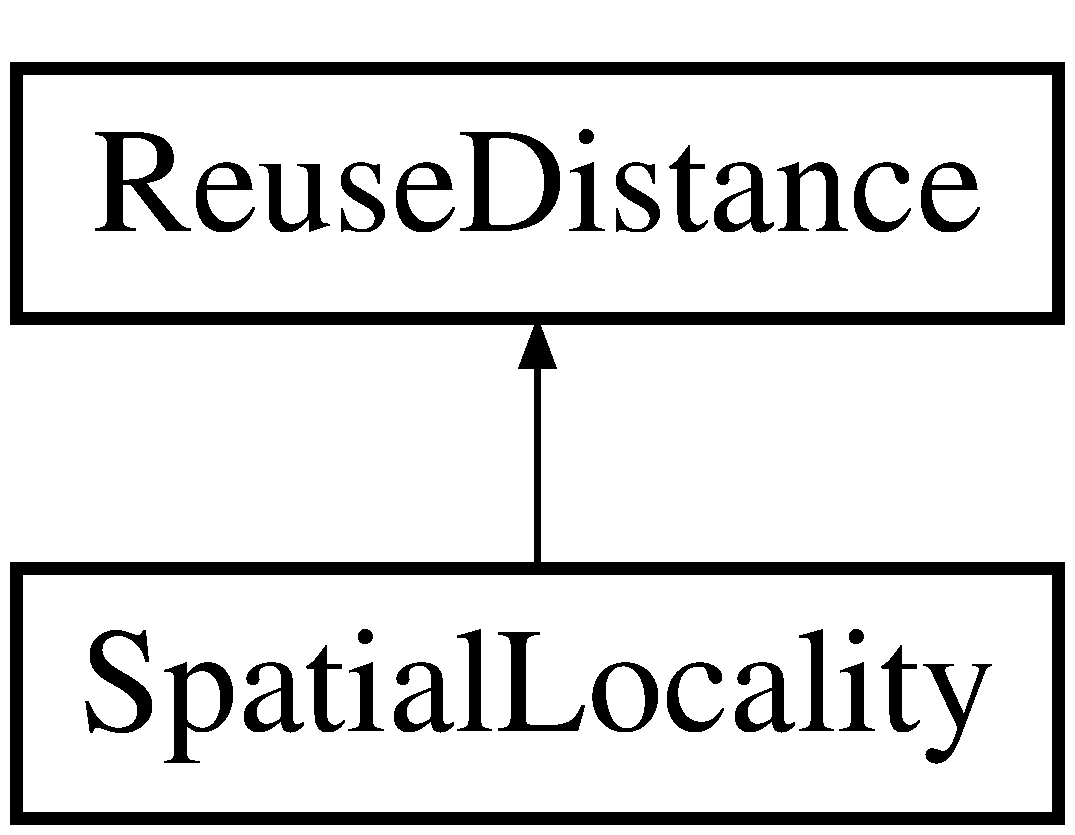
\includegraphics[height=2cm]{class_spatial_locality}
\end{center}
\end{figure}
\subsection*{Public Member Functions}
\begin{DoxyCompactItemize}
\item 
\hyperlink{class_spatial_locality_aff3106d38ff5ba3e6ecaec0c7214eaea}{SpatialLocality} (uint64\_\-t w, uint64\_\-t b, uint64\_\-t n)
\item 
\hyperlink{class_spatial_locality_a908469b7cd8a92c22a8bae4e2d4c5ade}{SpatialLocality} (uint64\_\-t w, uint64\_\-t b)
\item 
\hyperlink{class_spatial_locality_a63d45541023cfc370b079f1011cab5b8}{SpatialLocality} (uint64\_\-t w)
\item 
\hyperlink{class_spatial_locality_a449d21fbe63121ea92aaf5c1e0b8cb9c}{SpatialLocality} ()
\item 
virtual \hyperlink{class_spatial_locality_abfdaf3722786c5ad9ea65f885cbbebc6}{$\sim$SpatialLocality} ()
\item 
virtual void \hyperlink{class_spatial_locality_afef7ecfce7f238dbef37499e08edfb98}{GetActiveAddresses} (std::vector$<$ uint64\_\-t $>$ \&addrs)
\item 
virtual void \hyperlink{class_spatial_locality_a72a96a67e1791851927dbf3e5ceb206f}{Process} (\hyperlink{struct_reuse_entry}{ReuseEntry} \&addr)
\item 
virtual void \hyperlink{class_spatial_locality_acdfe7e6ac7891c4673cb7023af7227e0}{SkipAddresses} (uint64\_\-t amount)
\end{DoxyCompactItemize}
\subsection*{Static Public Attributes}
\begin{DoxyCompactItemize}
\item 
static const uint64\_\-t \hyperlink{class_spatial_locality_a563aa890ea539ae76c942fd1827a3095}{DefaultWindowSize} = 64
\end{DoxyCompactItemize}


\subsection{Detailed Description}
Finds and tracks spatial locality within a memory address stream. Spatial locality is defined as the minimum distance between the current address and any of the previous N addresses, as in \href{http://www.sdsc.edu/~allans/sc05_locality.pdf.}{\tt http://www.sdsc.edu/$\sim$allans/sc05\_\-locality.pdf.} This class allows that window size N to be customized. For basic usage, see the documentation at \href{http://bit.ly/ScqZVj}{\tt http://bit.ly/ScqZVj} for the constructors, the Process methods and the Print methods. Also see the simple test file test/test.cpp included in this source package. 

Definition at line 388 of file ReuseDistance.hpp.



\subsection{Constructor \& Destructor Documentation}
\hypertarget{class_spatial_locality_aff3106d38ff5ba3e6ecaec0c7214eaea}{
\index{SpatialLocality@{SpatialLocality}!SpatialLocality@{SpatialLocality}}
\index{SpatialLocality@{SpatialLocality}!SpatialLocality@{SpatialLocality}}
\subsubsection[{SpatialLocality}]{\setlength{\rightskip}{0pt plus 5cm}SpatialLocality::SpatialLocality (uint64\_\-t {\em w}, \/  uint64\_\-t {\em b}, \/  uint64\_\-t {\em n})\hspace{0.3cm}{\ttfamily  \mbox{[}inline\mbox{]}}}}
\label{class_spatial_locality_aff3106d38ff5ba3e6ecaec0c7214eaea}
Contructs a \hyperlink{class_reuse_distance}{ReuseDistance} object.


\begin{DoxyParams}{Parameters}
\item[{\em w}]The maximum window size, which is the maximum number of addresses that will be searched for spatial locality. w != \hyperlink{class_reuse_distance_a59f7f0ac6ad014472537619394ac7375}{ReuseDistance::Infinity} is enforced at runtime. \item[{\em b}]All distances not greater than b will be tracked individually. All distances are tracked individually if b == \hyperlink{class_reuse_distance_a59f7f0ac6ad014472537619394ac7375}{ReuseDistance::Infinity}. Beyond individual tracking, distances are tracked in bins whose boundaries are the powers of two greater than b and not greater than n. \item[{\em n}]All distances greater than n will be counted as infinite. Use n == \hyperlink{class_reuse_distance_a59f7f0ac6ad014472537619394ac7375}{ReuseDistance::Infinity} for no limit. n $>$= b is enforced at runtime. \end{DoxyParams}


Definition at line 420 of file ReuseDistance.hpp.

\hypertarget{class_spatial_locality_a908469b7cd8a92c22a8bae4e2d4c5ade}{
\index{SpatialLocality@{SpatialLocality}!SpatialLocality@{SpatialLocality}}
\index{SpatialLocality@{SpatialLocality}!SpatialLocality@{SpatialLocality}}
\subsubsection[{SpatialLocality}]{\setlength{\rightskip}{0pt plus 5cm}SpatialLocality::SpatialLocality (uint64\_\-t {\em w}, \/  uint64\_\-t {\em b})\hspace{0.3cm}{\ttfamily  \mbox{[}inline\mbox{]}}}}
\label{class_spatial_locality_a908469b7cd8a92c22a8bae4e2d4c5ade}
Constructs a \hyperlink{class_spatial_locality}{SpatialLocality} object. Equivalent to calling the other 3-\/argument constructor with n == \hyperlink{class_reuse_distance_a59f7f0ac6ad014472537619394ac7375}{ReuseDistance::Infinity} 

Definition at line 426 of file ReuseDistance.hpp.

\hypertarget{class_spatial_locality_a63d45541023cfc370b079f1011cab5b8}{
\index{SpatialLocality@{SpatialLocality}!SpatialLocality@{SpatialLocality}}
\index{SpatialLocality@{SpatialLocality}!SpatialLocality@{SpatialLocality}}
\subsubsection[{SpatialLocality}]{\setlength{\rightskip}{0pt plus 5cm}SpatialLocality::SpatialLocality (uint64\_\-t {\em w})\hspace{0.3cm}{\ttfamily  \mbox{[}inline\mbox{]}}}}
\label{class_spatial_locality_a63d45541023cfc370b079f1011cab5b8}
Constructs a \hyperlink{class_spatial_locality}{SpatialLocality} object. Equivalent to calling the other 3-\/argument constructor with w == b and n == \hyperlink{class_reuse_distance_a59f7f0ac6ad014472537619394ac7375}{ReuseDistance::Infinity} 

Definition at line 432 of file ReuseDistance.hpp.

\hypertarget{class_spatial_locality_a449d21fbe63121ea92aaf5c1e0b8cb9c}{
\index{SpatialLocality@{SpatialLocality}!SpatialLocality@{SpatialLocality}}
\index{SpatialLocality@{SpatialLocality}!SpatialLocality@{SpatialLocality}}
\subsubsection[{SpatialLocality}]{\setlength{\rightskip}{0pt plus 5cm}SpatialLocality::SpatialLocality ()\hspace{0.3cm}{\ttfamily  \mbox{[}inline\mbox{]}}}}
\label{class_spatial_locality_a449d21fbe63121ea92aaf5c1e0b8cb9c}
Constructs a \hyperlink{class_spatial_locality}{SpatialLocality} object. Equivalent to calling the other 3-\/argument constructor with w == b == \hyperlink{class_spatial_locality_a563aa890ea539ae76c942fd1827a3095}{SpatialLocality::DefaultWindowSize} and n == \hyperlink{class_reuse_distance_a59f7f0ac6ad014472537619394ac7375}{ReuseDistance::Infinity} 

Definition at line 438 of file ReuseDistance.hpp.

\hypertarget{class_spatial_locality_abfdaf3722786c5ad9ea65f885cbbebc6}{
\index{SpatialLocality@{SpatialLocality}!$\sim$SpatialLocality@{$\sim$SpatialLocality}}
\index{$\sim$SpatialLocality@{$\sim$SpatialLocality}!SpatialLocality@{SpatialLocality}}
\subsubsection[{$\sim$SpatialLocality}]{\setlength{\rightskip}{0pt plus 5cm}virtual SpatialLocality::$\sim$SpatialLocality ()\hspace{0.3cm}{\ttfamily  \mbox{[}inline, virtual\mbox{]}}}}
\label{class_spatial_locality_abfdaf3722786c5ad9ea65f885cbbebc6}
Destroys a \hyperlink{class_spatial_locality}{SpatialLocality} object. 

Definition at line 443 of file ReuseDistance.hpp.



\subsection{Member Function Documentation}
\hypertarget{class_spatial_locality_afef7ecfce7f238dbef37499e08edfb98}{
\index{SpatialLocality@{SpatialLocality}!GetActiveAddresses@{GetActiveAddresses}}
\index{GetActiveAddresses@{GetActiveAddresses}!SpatialLocality@{SpatialLocality}}
\subsubsection[{GetActiveAddresses}]{\setlength{\rightskip}{0pt plus 5cm}void SpatialLocality::GetActiveAddresses (std::vector$<$ uint64\_\-t $>$ \& {\em addrs})\hspace{0.3cm}{\ttfamily  \mbox{[}virtual\mbox{]}}}}
\label{class_spatial_locality_afef7ecfce7f238dbef37499e08edfb98}
Get a std::vector containing all of the addresses currently in this \hyperlink{class_spatial_locality}{SpatialLocality} object's active window.


\begin{DoxyParams}{Parameters}
\item[{\em addrs}]A std::vector which will contain the addresses. It is an error to pass this vector non-\/empty (that is addrs.size() == 0 is enforced at runtime).\end{DoxyParams}
\begin{DoxyReturn}{Returns}
none 
\end{DoxyReturn}


Reimplemented from \hyperlink{class_reuse_distance_acc4885040a8a518fc10b5aa4da7d777a}{ReuseDistance}.



Definition at line 460 of file ReuseDistance.cpp.

\hypertarget{class_spatial_locality_a72a96a67e1791851927dbf3e5ceb206f}{
\index{SpatialLocality@{SpatialLocality}!Process@{Process}}
\index{Process@{Process}!SpatialLocality@{SpatialLocality}}
\subsubsection[{Process}]{\setlength{\rightskip}{0pt plus 5cm}void SpatialLocality::Process ({\bf ReuseEntry} \& {\em addr})\hspace{0.3cm}{\ttfamily  \mbox{[}virtual\mbox{]}}}}
\label{class_spatial_locality_a72a96a67e1791851927dbf3e5ceb206f}
Process a single memory address.


\begin{DoxyParams}{Parameters}
\item[{\em addr}]The structure describing the memory address to process.\end{DoxyParams}
\begin{DoxyReturn}{Returns}
none 
\end{DoxyReturn}


Reimplemented from \hyperlink{class_reuse_distance_a4ff6b77022ce62e0fdefa5cc297b932a}{ReuseDistance}.



Definition at line 389 of file ReuseDistance.cpp.

\hypertarget{class_spatial_locality_acdfe7e6ac7891c4673cb7023af7227e0}{
\index{SpatialLocality@{SpatialLocality}!SkipAddresses@{SkipAddresses}}
\index{SkipAddresses@{SkipAddresses}!SpatialLocality@{SpatialLocality}}
\subsubsection[{SkipAddresses}]{\setlength{\rightskip}{0pt plus 5cm}void SpatialLocality::SkipAddresses (uint64\_\-t {\em amount})\hspace{0.3cm}{\ttfamily  \mbox{[}virtual\mbox{]}}}}
\label{class_spatial_locality_acdfe7e6ac7891c4673cb7023af7227e0}
Pretend that some number of addresses in the stream were skipped. Useful for intervel-\/based sampling. This has the effect of flushing the entire window.


\begin{DoxyParams}{Parameters}
\item[{\em amount}]The number of addresses to skip.\end{DoxyParams}
\begin{DoxyReturn}{Returns}
none 
\end{DoxyReturn}


Reimplemented from \hyperlink{class_reuse_distance_a0763528236db14a9e0234465e72da3b6}{ReuseDistance}.



Definition at line 441 of file ReuseDistance.cpp.



\subsection{Member Data Documentation}
\hypertarget{class_spatial_locality_a563aa890ea539ae76c942fd1827a3095}{
\index{SpatialLocality@{SpatialLocality}!DefaultWindowSize@{DefaultWindowSize}}
\index{DefaultWindowSize@{DefaultWindowSize}!SpatialLocality@{SpatialLocality}}
\subsubsection[{DefaultWindowSize}]{\setlength{\rightskip}{0pt plus 5cm}const uint64\_\-t {\bf SpatialLocality::DefaultWindowSize} = 64\hspace{0.3cm}{\ttfamily  \mbox{[}static\mbox{]}}}}
\label{class_spatial_locality_a563aa890ea539ae76c942fd1827a3095}


Definition at line 407 of file ReuseDistance.hpp.



The documentation for this class was generated from the following files:\begin{DoxyCompactItemize}
\item 
/home/michaell/software/ReuseDistance/\hyperlink{_reuse_distance_8hpp}{ReuseDistance.hpp}\item 
/home/michaell/software/ReuseDistance/\hyperlink{_reuse_distance_8cpp}{ReuseDistance.cpp}\end{DoxyCompactItemize}

\hypertarget{structtree234___tag}{
\section{tree234\_\-Tag Struct Reference}
\label{structtree234___tag}\index{tree234\_\-Tag@{tree234\_\-Tag}}
}
\subsection*{Public Attributes}
\begin{DoxyCompactItemize}
\item 
\hyperlink{structnode234___tag}{node234} $\ast$ \hyperlink{structtree234___tag_a87972e40a769f91133666daede8341de}{root}
\end{DoxyCompactItemize}


\subsection{Detailed Description}


Definition at line 54 of file tree234.c.



\subsection{Member Data Documentation}
\hypertarget{structtree234___tag_a87972e40a769f91133666daede8341de}{
\index{tree234\_\-Tag@{tree234\_\-Tag}!root@{root}}
\index{root@{root}!tree234_Tag@{tree234\_\-Tag}}
\subsubsection[{root}]{\setlength{\rightskip}{0pt plus 5cm}{\bf node234}$\ast$ {\bf tree234\_\-Tag::root}}}
\label{structtree234___tag_a87972e40a769f91133666daede8341de}


Definition at line 55 of file tree234.c.



The documentation for this struct was generated from the following file:\begin{DoxyCompactItemize}
\item 
/home/michaell/software/ReuseDistance/\hyperlink{tree234_8c}{tree234.c}\end{DoxyCompactItemize}

\chapter{File Documentation}
\hypertarget{foo_8cpp}{
\section{/home/michaell/software/ReuseDistance/foo.cpp File Reference}
\label{foo_8cpp}\index{/home/michaell/software/ReuseDistance/foo.cpp@{/home/michaell/software/ReuseDistance/foo.cpp}}
}
{\ttfamily \#include $<$map$>$}\par
{\ttfamily \#include $<$stdint.h$>$}\par
\subsection*{Functions}
\begin{DoxyCompactItemize}
\item 
int \hyperlink{foo_8cpp_a3c04138a5bfe5d72780bb7e82a18e627}{main} (int argc, char $\ast$$\ast$argv)
\end{DoxyCompactItemize}


\subsection{Function Documentation}
\hypertarget{foo_8cpp_a3c04138a5bfe5d72780bb7e82a18e627}{
\index{foo.cpp@{foo.cpp}!main@{main}}
\index{main@{main}!foo.cpp@{foo.cpp}}
\subsubsection[{main}]{\setlength{\rightskip}{0pt plus 5cm}int main (int {\em argc}, \/  char $\ast$$\ast$ {\em argv})}}
\label{foo_8cpp_a3c04138a5bfe5d72780bb7e82a18e627}


Definition at line 6 of file foo.cpp.


\hypertarget{_reuse_distance_8cpp}{
\section{/home/michaell/software/ReuseDistance/ReuseDistance.cpp File Reference}
\label{_reuse_distance_8cpp}\index{/home/michaell/software/ReuseDistance/ReuseDistance.cpp@{/home/michaell/software/ReuseDistance/ReuseDistance.cpp}}
}
{\ttfamily \#include $<$ReuseDistance.hpp$>$}\par
\subsection*{Defines}
\begin{DoxyCompactItemize}
\item 
\#define \hyperlink{_reuse_distance_8cpp_a3327767daab03e63eea2da98f879aeb0}{REUSE\_\-DEBUG}
\item 
\#define \hyperlink{_reuse_distance_8cpp_a9e8e006a667f063cebf15eead00b2bed}{debug\_\-assert}(...)~assert(\_\-\_\-VA\_\-ARGS\_\-\_\-)
\end{DoxyCompactItemize}
\subsection*{Functions}
\begin{DoxyCompactItemize}
\item 
uint64\_\-t \hyperlink{_reuse_distance_8cpp_acdb43500f09c3e4c1ffaa8366d5ce56f}{uint64abs} (uint64\_\-t a)
\item 
uint64\_\-t \hyperlink{_reuse_distance_8cpp_a91e4942b7d7024c35ea988504769b6cc}{ShaveBitsPwr2} (uint64\_\-t val)
\end{DoxyCompactItemize}


\subsection{Define Documentation}
\hypertarget{_reuse_distance_8cpp_a9e8e006a667f063cebf15eead00b2bed}{
\index{ReuseDistance.cpp@{ReuseDistance.cpp}!debug\_\-assert@{debug\_\-assert}}
\index{debug\_\-assert@{debug\_\-assert}!ReuseDistance.cpp@{ReuseDistance.cpp}}
\subsubsection[{debug\_\-assert}]{\setlength{\rightskip}{0pt plus 5cm}\#define debug\_\-assert( {\em ...})~assert(\_\-\_\-VA\_\-ARGS\_\-\_\-)}}
\label{_reuse_distance_8cpp_a9e8e006a667f063cebf15eead00b2bed}


Definition at line 27 of file ReuseDistance.cpp.

\hypertarget{_reuse_distance_8cpp_a3327767daab03e63eea2da98f879aeb0}{
\index{ReuseDistance.cpp@{ReuseDistance.cpp}!REUSE\_\-DEBUG@{REUSE\_\-DEBUG}}
\index{REUSE\_\-DEBUG@{REUSE\_\-DEBUG}!ReuseDistance.cpp@{ReuseDistance.cpp}}
\subsubsection[{REUSE\_\-DEBUG}]{\setlength{\rightskip}{0pt plus 5cm}\#define REUSE\_\-DEBUG}}
\label{_reuse_distance_8cpp_a3327767daab03e63eea2da98f879aeb0}


Definition at line 25 of file ReuseDistance.cpp.



\subsection{Function Documentation}
\hypertarget{_reuse_distance_8cpp_a91e4942b7d7024c35ea988504769b6cc}{
\index{ReuseDistance.cpp@{ReuseDistance.cpp}!ShaveBitsPwr2@{ShaveBitsPwr2}}
\index{ShaveBitsPwr2@{ShaveBitsPwr2}!ReuseDistance.cpp@{ReuseDistance.cpp}}
\subsubsection[{ShaveBitsPwr2}]{\setlength{\rightskip}{0pt plus 5cm}uint64\_\-t ShaveBitsPwr2 (uint64\_\-t {\em val})\hspace{0.3cm}{\ttfamily  \mbox{[}inline\mbox{]}}}}
\label{_reuse_distance_8cpp_a91e4942b7d7024c35ea988504769b6cc}


Definition at line 271 of file ReuseDistance.cpp.

\hypertarget{_reuse_distance_8cpp_acdb43500f09c3e4c1ffaa8366d5ce56f}{
\index{ReuseDistance.cpp@{ReuseDistance.cpp}!uint64abs@{uint64abs}}
\index{uint64abs@{uint64abs}!ReuseDistance.cpp@{ReuseDistance.cpp}}
\subsubsection[{uint64abs}]{\setlength{\rightskip}{0pt plus 5cm}uint64\_\-t uint64abs (uint64\_\-t {\em a})\hspace{0.3cm}{\ttfamily  \mbox{[}inline\mbox{]}}}}
\label{_reuse_distance_8cpp_acdb43500f09c3e4c1ffaa8366d5ce56f}


Definition at line 32 of file ReuseDistance.cpp.


\hypertarget{_reuse_distance_8hpp}{
\section{/home/michaell/software/ReuseDistance/ReuseDistance.hpp File Reference}
\label{_reuse_distance_8hpp}\index{/home/michaell/software/ReuseDistance/ReuseDistance.hpp@{/home/michaell/software/ReuseDistance/ReuseDistance.hpp}}
}
{\ttfamily \#include $<$assert.h$>$}\par
{\ttfamily \#include $<$stdlib.h$>$}\par
{\ttfamily \#include $<$tree234.h$>$}\par
{\ttfamily \#include $<$algorithm$>$}\par
{\ttfamily \#include $<$iostream$>$}\par
{\ttfamily \#include $<$ostream$>$}\par
{\ttfamily \#include $<$list$>$}\par
{\ttfamily \#include $<$map$>$}\par
{\ttfamily \#include $<$vector$>$}\par
\subsection*{Classes}
\begin{DoxyCompactItemize}
\item 
struct \hyperlink{struct_reuse_entry}{ReuseEntry}
\item 
class \hyperlink{class_reuse_distance}{ReuseDistance}
\item 
class \hyperlink{class_reuse_stats}{ReuseStats}
\item 
class \hyperlink{class_spatial_locality}{SpatialLocality}
\end{DoxyCompactItemize}
\subsection*{Defines}
\begin{DoxyCompactItemize}
\item 
\#define \hyperlink{_reuse_distance_8hpp_ae458bf0a7bac23a65b544ba5000f1417}{reuse\_\-map\_\-type}~std::map
\item 
\#define \hyperlink{_reuse_distance_8hpp_ad58a1fbfc85c7e4790fc55e654f50221}{TAB}~\char`\"{}$\backslash$t\char`\"{}
\item 
\#define \hyperlink{_reuse_distance_8hpp_a90dc3f3ee970394e0080300526390a84}{ENDL}~\char`\"{}$\backslash$n\char`\"{}
\item 
\#define \hyperlink{_reuse_distance_8hpp_aebf444a7be286ab578986a907fdb0c02}{\_\-\_\-seq}~id
\item 
\#define \hyperlink{_reuse_distance_8hpp_a3bb9d1622c7f1c40306b84e0016af365}{INFINITY\_\-REUSE}~(0)
\item 
\#define \hyperlink{_reuse_distance_8hpp_ab5fb19d7ada3431a22245b01c341584e}{INVALID\_\-SPATIAL}~(0xFFFFFFFFFFFFFFFFL)
\end{DoxyCompactItemize}
\subsection*{Functions}
\begin{DoxyCompactItemize}
\item 
int \hyperlink{_reuse_distance_8hpp_abd5d231354fc09eb8b735eccdc1f2408}{reusecmp} (void $\ast$va, void $\ast$vb)
\end{DoxyCompactItemize}


\subsection{Detailed Description}
\begin{DoxyAuthor}{Author}
Michael Laurenzano $<$\href{mailto:michaell@sdsc.edu}{\tt michaell@sdsc.edu}$>$ 
\end{DoxyAuthor}
\begin{DoxyVersion}{Version}
0.01
\end{DoxyVersion}
\hypertarget{_reuse_distance_8hpp_LICENSE}{}\subsection{LICENSE}\label{_reuse_distance_8hpp_LICENSE}
This file is part of the \hyperlink{class_reuse_distance}{ReuseDistance} tool.

Copyright (c) 2012, University of California Regents All rights reserved.

This program is free software: you can redistribute it and/or modify it under the terms of the GNU General Public License as published by the Free Software Foundation, either version 3 of the License, or (at your option) any later version.

This program is distributed in the hope that it will be useful, but WITHOUT ANY WARRANTY; without even the implied warranty of MERCHANTABILITY or FITNESS FOR A PARTICULAR PURPOSE. See the GNU General Public License for more details.

You should have received a copy of the GNU General Public License along with this program. If not, see $<$\href{http://www.gnu.org/licenses/}{\tt http://www.gnu.org/licenses/}$>$.\hypertarget{_reuse_distance_8hpp_DESCRIPTION}{}\subsection{DESCRIPTION}\label{_reuse_distance_8hpp_DESCRIPTION}
The ReuseDistanceHandler class allows for calculation and statistic tracking for finding memory reuse distances given a stream of memory addresses and ids. 

Definition in file \hyperlink{_reuse_distance_8hpp_source}{ReuseDistance.hpp}.



\subsection{Define Documentation}
\hypertarget{_reuse_distance_8hpp_aebf444a7be286ab578986a907fdb0c02}{
\index{ReuseDistance.hpp@{ReuseDistance.hpp}!\_\-\_\-seq@{\_\-\_\-seq}}
\index{\_\-\_\-seq@{\_\-\_\-seq}!ReuseDistance.hpp@{ReuseDistance.hpp}}
\subsubsection[{\_\-\_\-seq}]{\setlength{\rightskip}{0pt plus 5cm}\#define \_\-\_\-seq~id}}
\label{_reuse_distance_8hpp_aebf444a7be286ab578986a907fdb0c02}


Definition at line 54 of file ReuseDistance.hpp.

\hypertarget{_reuse_distance_8hpp_a90dc3f3ee970394e0080300526390a84}{
\index{ReuseDistance.hpp@{ReuseDistance.hpp}!ENDL@{ENDL}}
\index{ENDL@{ENDL}!ReuseDistance.hpp@{ReuseDistance.hpp}}
\subsubsection[{ENDL}]{\setlength{\rightskip}{0pt plus 5cm}\#define ENDL~\char`\"{}$\backslash$n\char`\"{}}}
\label{_reuse_distance_8hpp_a90dc3f3ee970394e0080300526390a84}


Definition at line 52 of file ReuseDistance.hpp.

\hypertarget{_reuse_distance_8hpp_a3bb9d1622c7f1c40306b84e0016af365}{
\index{ReuseDistance.hpp@{ReuseDistance.hpp}!INFINITY\_\-REUSE@{INFINITY\_\-REUSE}}
\index{INFINITY\_\-REUSE@{INFINITY\_\-REUSE}!ReuseDistance.hpp@{ReuseDistance.hpp}}
\subsubsection[{INFINITY\_\-REUSE}]{\setlength{\rightskip}{0pt plus 5cm}\#define INFINITY\_\-REUSE~(0)}}
\label{_reuse_distance_8hpp_a3bb9d1622c7f1c40306b84e0016af365}


Definition at line 57 of file ReuseDistance.hpp.

\hypertarget{_reuse_distance_8hpp_ab5fb19d7ada3431a22245b01c341584e}{
\index{ReuseDistance.hpp@{ReuseDistance.hpp}!INVALID\_\-SPATIAL@{INVALID\_\-SPATIAL}}
\index{INVALID\_\-SPATIAL@{INVALID\_\-SPATIAL}!ReuseDistance.hpp@{ReuseDistance.hpp}}
\subsubsection[{INVALID\_\-SPATIAL}]{\setlength{\rightskip}{0pt plus 5cm}\#define INVALID\_\-SPATIAL~(0xFFFFFFFFFFFFFFFFL)}}
\label{_reuse_distance_8hpp_ab5fb19d7ada3431a22245b01c341584e}


Definition at line 58 of file ReuseDistance.hpp.

\hypertarget{_reuse_distance_8hpp_ae458bf0a7bac23a65b544ba5000f1417}{
\index{ReuseDistance.hpp@{ReuseDistance.hpp}!reuse\_\-map\_\-type@{reuse\_\-map\_\-type}}
\index{reuse\_\-map\_\-type@{reuse\_\-map\_\-type}!ReuseDistance.hpp@{ReuseDistance.hpp}}
\subsubsection[{reuse\_\-map\_\-type}]{\setlength{\rightskip}{0pt plus 5cm}\#define reuse\_\-map\_\-type~std::map}}
\label{_reuse_distance_8hpp_ae458bf0a7bac23a65b544ba5000f1417}


Definition at line 48 of file ReuseDistance.hpp.

\hypertarget{_reuse_distance_8hpp_ad58a1fbfc85c7e4790fc55e654f50221}{
\index{ReuseDistance.hpp@{ReuseDistance.hpp}!TAB@{TAB}}
\index{TAB@{TAB}!ReuseDistance.hpp@{ReuseDistance.hpp}}
\subsubsection[{TAB}]{\setlength{\rightskip}{0pt plus 5cm}\#define TAB~\char`\"{}$\backslash$t\char`\"{}}}
\label{_reuse_distance_8hpp_ad58a1fbfc85c7e4790fc55e654f50221}


Definition at line 51 of file ReuseDistance.hpp.



\subsection{Function Documentation}
\hypertarget{_reuse_distance_8hpp_abd5d231354fc09eb8b735eccdc1f2408}{
\index{ReuseDistance.hpp@{ReuseDistance.hpp}!reusecmp@{reusecmp}}
\index{reusecmp@{reusecmp}!ReuseDistance.hpp@{ReuseDistance.hpp}}
\subsubsection[{reusecmp}]{\setlength{\rightskip}{0pt plus 5cm}int reusecmp (void $\ast$ {\em va}, \/  void $\ast$ {\em vb})}}
\label{_reuse_distance_8hpp_abd5d231354fc09eb8b735eccdc1f2408}

\hypertarget{tree234_8c}{
\section{/home/michaell/software/ReuseDistance/tree234.c File Reference}
\label{tree234_8c}\index{/home/michaell/software/ReuseDistance/tree234.c@{/home/michaell/software/ReuseDistance/tree234.c}}
}
{\ttfamily \#include $<$stdio.h$>$}\par
{\ttfamily \#include $<$stdlib.h$>$}\par
{\ttfamily \#include $<$assert.h$>$}\par
{\ttfamily \#include \char`\"{}tree234.h\char`\"{}}\par
{\ttfamily \#include $<$tree234.h$>$}\par
{\ttfamily \#include $<$algorithm$>$}\par
{\ttfamily \#include $<$iostream$>$}\par
{\ttfamily \#include $<$ostream$>$}\par
{\ttfamily \#include $<$list$>$}\par
{\ttfamily \#include $<$map$>$}\par
{\ttfamily \#include $<$vector$>$}\par
\subsection*{Classes}
\begin{DoxyCompactItemize}
\item 
struct \hyperlink{structtree234___tag}{tree234\_\-Tag}
\item 
struct \hyperlink{structnode234___tag}{node234\_\-Tag}
\end{DoxyCompactItemize}
\subsection*{Defines}
\begin{DoxyCompactItemize}
\item 
\#define \hyperlink{tree234_8c_afcd8de4bd7906015024bbf95d3af04b8}{smalloc}~malloc
\item 
\#define \hyperlink{tree234_8c_ada7df53d3be111d15cfc15301a8fd916}{sfree}~free
\item 
\#define \hyperlink{tree234_8c_a8f2e94fbea31b57401440dfa50c63614}{mknew}(typ)~( (typ $\ast$) smalloc (sizeof (typ)) )
\item 
\#define \hyperlink{tree234_8c_af855c94dc540e943632089ce7496faac}{LOG}(x)
\item 
\#define \hyperlink{tree234_8c_aebd6de699a670101f0c811e2f09af9f6}{reusecmp}(va, vb)~(va-\/$>$\_\-\_\-seq -\/ vb-\/$>$\_\-\_\-seq)
\end{DoxyCompactItemize}
\subsection*{Typedefs}
\begin{DoxyCompactItemize}
\item 
typedef struct \hyperlink{structnode234___tag}{node234\_\-Tag} \hyperlink{tree234_8c_ab77f4958aafc99545a0299a1d8025669}{node234}
\end{DoxyCompactItemize}
\subsection*{Functions}
\begin{DoxyCompactItemize}
\item 
\hyperlink{structtree234___tag}{tree234} $\ast$ \hyperlink{tree234_8c_ae664a1e477b5e7f8393066ff3b285d29}{newtree234} ()
\item 
void \hyperlink{tree234_8c_a122e9c343f78e9962779515d45b25519}{freetree234} (\hyperlink{structtree234___tag}{tree234} $\ast$t)
\item 
int \hyperlink{tree234_8c_ae895b57010fce40245e400b5ca0a863d}{count234} (\hyperlink{structtree234___tag}{tree234} $\ast$t)
\item 
\hyperlink{struct_reuse_entry}{ReuseEntry} $\ast$ \hyperlink{tree234_8c_a1140d7d14c9b9b2baed0242ff0f270f8}{add234} (\hyperlink{structtree234___tag}{tree234} $\ast$t, \hyperlink{struct_reuse_entry}{ReuseEntry} $\ast$e)
\item 
\hyperlink{struct_reuse_entry}{ReuseEntry} $\ast$ \hyperlink{tree234_8c_ace1d0830e7caf3f0300165175e6223a5}{index234} (\hyperlink{structtree234___tag}{tree234} $\ast$t, int index)
\item 
\hyperlink{struct_reuse_entry}{ReuseEntry} $\ast$ \hyperlink{tree234_8c_aa0f45120b68ef1f1e29ce95d91c6fa9f}{findrelpos234} (\hyperlink{structtree234___tag}{tree234} $\ast$t, \hyperlink{struct_reuse_entry}{ReuseEntry} $\ast$e, int $\ast$index)
\item 
\hyperlink{struct_reuse_entry}{ReuseEntry} $\ast$ \hyperlink{tree234_8c_a00ed8a6a79cee600be3a197d14f3a9c5}{delpos234} (\hyperlink{structtree234___tag}{tree234} $\ast$t, int index)
\item 
\hyperlink{struct_reuse_entry}{ReuseEntry} $\ast$ \hyperlink{tree234_8c_a0d1b312731d003e68a8ebdfa9350641c}{del234} (\hyperlink{structtree234___tag}{tree234} $\ast$t, \hyperlink{struct_reuse_entry}{ReuseEntry} $\ast$e)
\end{DoxyCompactItemize}


\subsection{Define Documentation}
\hypertarget{tree234_8c_af855c94dc540e943632089ce7496faac}{
\index{tree234.c@{tree234.c}!LOG@{LOG}}
\index{LOG@{LOG}!tree234.c@{tree234.c}}
\subsubsection[{LOG}]{\setlength{\rightskip}{0pt plus 5cm}\#define LOG(x)}}
\label{tree234_8c_af855c94dc540e943632089ce7496faac}


Definition at line 47 of file tree234.c.

\hypertarget{tree234_8c_a8f2e94fbea31b57401440dfa50c63614}{
\index{tree234.c@{tree234.c}!mknew@{mknew}}
\index{mknew@{mknew}!tree234.c@{tree234.c}}
\subsubsection[{mknew}]{\setlength{\rightskip}{0pt plus 5cm}\#define mknew(typ)~( (typ $\ast$) smalloc (sizeof (typ)) )}}
\label{tree234_8c_a8f2e94fbea31b57401440dfa50c63614}


Definition at line 42 of file tree234.c.

\hypertarget{tree234_8c_aebd6de699a670101f0c811e2f09af9f6}{
\index{tree234.c@{tree234.c}!reusecmp@{reusecmp}}
\index{reusecmp@{reusecmp}!tree234.c@{tree234.c}}
\subsubsection[{reusecmp}]{\setlength{\rightskip}{0pt plus 5cm}\#define reusecmp(va, \/  vb)~(va-\/$>$\_\-\_\-seq -\/ vb-\/$>$\_\-\_\-seq)}}
\label{tree234_8c_aebd6de699a670101f0c811e2f09af9f6}


Definition at line 50 of file tree234.c.

\hypertarget{tree234_8c_ada7df53d3be111d15cfc15301a8fd916}{
\index{tree234.c@{tree234.c}!sfree@{sfree}}
\index{sfree@{sfree}!tree234.c@{tree234.c}}
\subsubsection[{sfree}]{\setlength{\rightskip}{0pt plus 5cm}\#define sfree~free}}
\label{tree234_8c_ada7df53d3be111d15cfc15301a8fd916}


Definition at line 40 of file tree234.c.

\hypertarget{tree234_8c_afcd8de4bd7906015024bbf95d3af04b8}{
\index{tree234.c@{tree234.c}!smalloc@{smalloc}}
\index{smalloc@{smalloc}!tree234.c@{tree234.c}}
\subsubsection[{smalloc}]{\setlength{\rightskip}{0pt plus 5cm}\#define smalloc~malloc}}
\label{tree234_8c_afcd8de4bd7906015024bbf95d3af04b8}


Definition at line 39 of file tree234.c.



\subsection{Typedef Documentation}
\hypertarget{tree234_8c_ab77f4958aafc99545a0299a1d8025669}{
\index{tree234.c@{tree234.c}!node234@{node234}}
\index{node234@{node234}!tree234.c@{tree234.c}}
\subsubsection[{node234}]{\setlength{\rightskip}{0pt plus 5cm}typedef struct {\bf node234\_\-Tag} {\bf node234}}}
\label{tree234_8c_ab77f4958aafc99545a0299a1d8025669}


Definition at line 52 of file tree234.c.



\subsection{Function Documentation}
\hypertarget{tree234_8c_a1140d7d14c9b9b2baed0242ff0f270f8}{
\index{tree234.c@{tree234.c}!add234@{add234}}
\index{add234@{add234}!tree234.c@{tree234.c}}
\subsubsection[{add234}]{\setlength{\rightskip}{0pt plus 5cm}{\bf ReuseEntry}$\ast$ add234 ({\bf tree234} $\ast$ {\em t}, \/  {\bf ReuseEntry} $\ast$ {\em e})}}
\label{tree234_8c_a1140d7d14c9b9b2baed0242ff0f270f8}


Definition at line 394 of file tree234.c.

\hypertarget{tree234_8c_ae895b57010fce40245e400b5ca0a863d}{
\index{tree234.c@{tree234.c}!count234@{count234}}
\index{count234@{count234}!tree234.c@{tree234.c}}
\subsubsection[{count234}]{\setlength{\rightskip}{0pt plus 5cm}int count234 ({\bf tree234} $\ast$ {\em t})}}
\label{tree234_8c_ae895b57010fce40245e400b5ca0a863d}


Definition at line 111 of file tree234.c.

\hypertarget{tree234_8c_a0d1b312731d003e68a8ebdfa9350641c}{
\index{tree234.c@{tree234.c}!del234@{del234}}
\index{del234@{del234}!tree234.c@{tree234.c}}
\subsubsection[{del234}]{\setlength{\rightskip}{0pt plus 5cm}{\bf ReuseEntry}$\ast$ del234 ({\bf tree234} $\ast$ {\em t}, \/  {\bf ReuseEntry} $\ast$ {\em e})}}
\label{tree234_8c_a0d1b312731d003e68a8ebdfa9350641c}


Definition at line 836 of file tree234.c.

\hypertarget{tree234_8c_a00ed8a6a79cee600be3a197d14f3a9c5}{
\index{tree234.c@{tree234.c}!delpos234@{delpos234}}
\index{delpos234@{delpos234}!tree234.c@{tree234.c}}
\subsubsection[{delpos234}]{\setlength{\rightskip}{0pt plus 5cm}{\bf ReuseEntry}$\ast$ delpos234 ({\bf tree234} $\ast$ {\em t}, \/  int {\em index})}}
\label{tree234_8c_a00ed8a6a79cee600be3a197d14f3a9c5}


Definition at line 830 of file tree234.c.

\hypertarget{tree234_8c_aa0f45120b68ef1f1e29ce95d91c6fa9f}{
\index{tree234.c@{tree234.c}!findrelpos234@{findrelpos234}}
\index{findrelpos234@{findrelpos234}!tree234.c@{tree234.c}}
\subsubsection[{findrelpos234}]{\setlength{\rightskip}{0pt plus 5cm}{\bf ReuseEntry}$\ast$ findrelpos234 ({\bf tree234} $\ast$ {\em t}, \/  {\bf ReuseEntry} $\ast$ {\em e}, \/  int $\ast$ {\em index})}}
\label{tree234_8c_aa0f45120b68ef1f1e29ce95d91c6fa9f}


Definition at line 441 of file tree234.c.

\hypertarget{tree234_8c_a122e9c343f78e9962779515d45b25519}{
\index{tree234.c@{tree234.c}!freetree234@{freetree234}}
\index{freetree234@{freetree234}!tree234.c@{tree234.c}}
\subsubsection[{freetree234}]{\setlength{\rightskip}{0pt plus 5cm}void freetree234 ({\bf tree234} $\ast$ {\em t})}}
\label{tree234_8c_a122e9c343f78e9962779515d45b25519}


Definition at line 87 of file tree234.c.

\hypertarget{tree234_8c_ace1d0830e7caf3f0300165175e6223a5}{
\index{tree234.c@{tree234.c}!index234@{index234}}
\index{index234@{index234}!tree234.c@{tree234.c}}
\subsubsection[{index234}]{\setlength{\rightskip}{0pt plus 5cm}{\bf ReuseEntry}$\ast$ index234 ({\bf tree234} $\ast$ {\em t}, \/  int {\em index})}}
\label{tree234_8c_ace1d0830e7caf3f0300165175e6223a5}


Definition at line 402 of file tree234.c.

\hypertarget{tree234_8c_ae664a1e477b5e7f8393066ff3b285d29}{
\index{tree234.c@{tree234.c}!newtree234@{newtree234}}
\index{newtree234@{newtree234}!tree234.c@{tree234.c}}
\subsubsection[{newtree234}]{\setlength{\rightskip}{0pt plus 5cm}{\bf tree234}$\ast$ newtree234 ()}}
\label{tree234_8c_ae664a1e477b5e7f8393066ff3b285d29}


Definition at line 68 of file tree234.c.


\hypertarget{tree234_8h}{
\section{/home/michaell/software/ReuseDistance/tree234.h File Reference}
\label{tree234_8h}\index{/home/michaell/software/ReuseDistance/tree234.h@{/home/michaell/software/ReuseDistance/tree234.h}}
}
\subsection*{Typedefs}
\begin{DoxyCompactItemize}
\item 
typedef struct \hyperlink{structtree234___tag}{tree234\_\-Tag} \hyperlink{tree234_8h_ac74d1aa8f2a6305539cda73718a367fa}{tree234}
\end{DoxyCompactItemize}
\subsection*{Functions}
\begin{DoxyCompactItemize}
\item 
\hyperlink{structtree234___tag}{tree234} $\ast$ \hyperlink{tree234_8h_ae664a1e477b5e7f8393066ff3b285d29}{newtree234} ()
\item 
void \hyperlink{tree234_8h_a122e9c343f78e9962779515d45b25519}{freetree234} (\hyperlink{structtree234___tag}{tree234} $\ast$t)
\item 
\hyperlink{struct_reuse_entry}{ReuseEntry} $\ast$ \hyperlink{tree234_8h_a1140d7d14c9b9b2baed0242ff0f270f8}{add234} (\hyperlink{structtree234___tag}{tree234} $\ast$t, \hyperlink{struct_reuse_entry}{ReuseEntry} $\ast$e)
\item 
\hyperlink{struct_reuse_entry}{ReuseEntry} $\ast$ \hyperlink{tree234_8h_abb942f2e8c39594c87e6bd4284ecd51a}{addpos234} (\hyperlink{structtree234___tag}{tree234} $\ast$t, \hyperlink{struct_reuse_entry}{ReuseEntry} $\ast$e, int index)
\item 
\hyperlink{struct_reuse_entry}{ReuseEntry} $\ast$ \hyperlink{tree234_8h_ace1d0830e7caf3f0300165175e6223a5}{index234} (\hyperlink{structtree234___tag}{tree234} $\ast$t, int index)
\item 
\hyperlink{struct_reuse_entry}{ReuseEntry} $\ast$ \hyperlink{tree234_8h_aa0f45120b68ef1f1e29ce95d91c6fa9f}{findrelpos234} (\hyperlink{structtree234___tag}{tree234} $\ast$t, \hyperlink{struct_reuse_entry}{ReuseEntry} $\ast$e, int $\ast$index)
\item 
\hyperlink{struct_reuse_entry}{ReuseEntry} $\ast$ \hyperlink{tree234_8h_a0d1b312731d003e68a8ebdfa9350641c}{del234} (\hyperlink{structtree234___tag}{tree234} $\ast$t, \hyperlink{struct_reuse_entry}{ReuseEntry} $\ast$e)
\item 
\hyperlink{struct_reuse_entry}{ReuseEntry} $\ast$ \hyperlink{tree234_8h_a00ed8a6a79cee600be3a197d14f3a9c5}{delpos234} (\hyperlink{structtree234___tag}{tree234} $\ast$t, int index)
\item 
int \hyperlink{tree234_8h_ae895b57010fce40245e400b5ca0a863d}{count234} (\hyperlink{structtree234___tag}{tree234} $\ast$t)
\end{DoxyCompactItemize}


\subsection{Typedef Documentation}
\hypertarget{tree234_8h_ac74d1aa8f2a6305539cda73718a367fa}{
\index{tree234.h@{tree234.h}!tree234@{tree234}}
\index{tree234@{tree234}!tree234.h@{tree234.h}}
\subsubsection[{tree234}]{\setlength{\rightskip}{0pt plus 5cm}typedef struct {\bf tree234\_\-Tag} {\bf tree234}}}
\label{tree234_8h_ac74d1aa8f2a6305539cda73718a367fa}


Definition at line 36 of file tree234.h.



\subsection{Function Documentation}
\hypertarget{tree234_8h_a1140d7d14c9b9b2baed0242ff0f270f8}{
\index{tree234.h@{tree234.h}!add234@{add234}}
\index{add234@{add234}!tree234.h@{tree234.h}}
\subsubsection[{add234}]{\setlength{\rightskip}{0pt plus 5cm}{\bf ReuseEntry}$\ast$ add234 ({\bf tree234} $\ast$ {\em t}, \/  {\bf ReuseEntry} $\ast$ {\em e})}}
\label{tree234_8h_a1140d7d14c9b9b2baed0242ff0f270f8}


Definition at line 394 of file tree234.c.

\hypertarget{tree234_8h_abb942f2e8c39594c87e6bd4284ecd51a}{
\index{tree234.h@{tree234.h}!addpos234@{addpos234}}
\index{addpos234@{addpos234}!tree234.h@{tree234.h}}
\subsubsection[{addpos234}]{\setlength{\rightskip}{0pt plus 5cm}{\bf ReuseEntry}$\ast$ addpos234 ({\bf tree234} $\ast$ {\em t}, \/  {\bf ReuseEntry} $\ast$ {\em e}, \/  int {\em index})}}
\label{tree234_8h_abb942f2e8c39594c87e6bd4284ecd51a}
\hypertarget{tree234_8h_ae895b57010fce40245e400b5ca0a863d}{
\index{tree234.h@{tree234.h}!count234@{count234}}
\index{count234@{count234}!tree234.h@{tree234.h}}
\subsubsection[{count234}]{\setlength{\rightskip}{0pt plus 5cm}int count234 ({\bf tree234} $\ast$ {\em t})}}
\label{tree234_8h_ae895b57010fce40245e400b5ca0a863d}


Definition at line 111 of file tree234.c.

\hypertarget{tree234_8h_a0d1b312731d003e68a8ebdfa9350641c}{
\index{tree234.h@{tree234.h}!del234@{del234}}
\index{del234@{del234}!tree234.h@{tree234.h}}
\subsubsection[{del234}]{\setlength{\rightskip}{0pt plus 5cm}{\bf ReuseEntry}$\ast$ del234 ({\bf tree234} $\ast$ {\em t}, \/  {\bf ReuseEntry} $\ast$ {\em e})}}
\label{tree234_8h_a0d1b312731d003e68a8ebdfa9350641c}


Definition at line 836 of file tree234.c.

\hypertarget{tree234_8h_a00ed8a6a79cee600be3a197d14f3a9c5}{
\index{tree234.h@{tree234.h}!delpos234@{delpos234}}
\index{delpos234@{delpos234}!tree234.h@{tree234.h}}
\subsubsection[{delpos234}]{\setlength{\rightskip}{0pt plus 5cm}{\bf ReuseEntry}$\ast$ delpos234 ({\bf tree234} $\ast$ {\em t}, \/  int {\em index})}}
\label{tree234_8h_a00ed8a6a79cee600be3a197d14f3a9c5}


Definition at line 830 of file tree234.c.

\hypertarget{tree234_8h_aa0f45120b68ef1f1e29ce95d91c6fa9f}{
\index{tree234.h@{tree234.h}!findrelpos234@{findrelpos234}}
\index{findrelpos234@{findrelpos234}!tree234.h@{tree234.h}}
\subsubsection[{findrelpos234}]{\setlength{\rightskip}{0pt plus 5cm}{\bf ReuseEntry}$\ast$ findrelpos234 ({\bf tree234} $\ast$ {\em t}, \/  {\bf ReuseEntry} $\ast$ {\em e}, \/  int $\ast$ {\em index})}}
\label{tree234_8h_aa0f45120b68ef1f1e29ce95d91c6fa9f}


Definition at line 441 of file tree234.c.

\hypertarget{tree234_8h_a122e9c343f78e9962779515d45b25519}{
\index{tree234.h@{tree234.h}!freetree234@{freetree234}}
\index{freetree234@{freetree234}!tree234.h@{tree234.h}}
\subsubsection[{freetree234}]{\setlength{\rightskip}{0pt plus 5cm}void freetree234 ({\bf tree234} $\ast$ {\em t})}}
\label{tree234_8h_a122e9c343f78e9962779515d45b25519}


Definition at line 87 of file tree234.c.

\hypertarget{tree234_8h_ace1d0830e7caf3f0300165175e6223a5}{
\index{tree234.h@{tree234.h}!index234@{index234}}
\index{index234@{index234}!tree234.h@{tree234.h}}
\subsubsection[{index234}]{\setlength{\rightskip}{0pt plus 5cm}{\bf ReuseEntry}$\ast$ index234 ({\bf tree234} $\ast$ {\em t}, \/  int {\em index})}}
\label{tree234_8h_ace1d0830e7caf3f0300165175e6223a5}


Definition at line 402 of file tree234.c.

\hypertarget{tree234_8h_ae664a1e477b5e7f8393066ff3b285d29}{
\index{tree234.h@{tree234.h}!newtree234@{newtree234}}
\index{newtree234@{newtree234}!tree234.h@{tree234.h}}
\subsubsection[{newtree234}]{\setlength{\rightskip}{0pt plus 5cm}{\bf tree234}$\ast$ newtree234 ()}}
\label{tree234_8h_ae664a1e477b5e7f8393066ff3b285d29}


Definition at line 68 of file tree234.c.


\printindex
\end{document}
